\documentclass[11pt]{article}

\usepackage[utf8]{inputenc}
\IfFileExists{lmodern.sty}{\usepackage[T1]{fontenc}\usepackage{lmodern}}{}
\usepackage{amsmath,amssymb,amsthm,mathtools}
\usepackage{booktabs}
\usepackage{microtype}
\usepackage[margin=1.05in]{geometry}
\usepackage{enumitem}
\usepackage{xcolor}
\usepackage{tikz}
\usetikzlibrary{arrows.meta,calc,positioning,decorations.pathreplacing}
\usepackage{pgfplots}
\pgfplotsset{compat=1.18}
\usepgfplotslibrary{fillbetween,groupplots}
\usepackage[most]{tcolorbox}
\usepackage[colorlinks=true,linkcolor=blue!55!black,citecolor=blue!55!black,urlcolor=blue!55!black]{hyperref}
\usepackage[nameinlink,capitalise]{cleveref}

\newtheorem{theorem}{Theorem}[section]
\newtheorem{proposition}[theorem]{Proposition}
\newtheorem{lemma}[theorem]{Lemma}
\newtheorem{corollary}[theorem]{Corollary}
\newtheorem{mainthm}{Theorem}
\renewcommand{\themainthm}{\Alph{mainthm}}
\newtheorem*{pentcor}{Corollary (the Duan--Winter pentagon conjecture)}
\theoremstyle{definition}
\newtheorem{definition}[theorem]{Definition}
\newtheorem{remark}[theorem]{Remark}
\crefname{mainthm}{Theorem}{Theorems}

\DeclareMathOperator{\Tr}{Tr}
\DeclareMathOperator{\supp}{supp}
\DeclareMathOperator{\ran}{ran}
\DeclareMathOperator{\vect}{vec}

\newcommand{\vt}{\vartheta}
\newcommand{\cH}{\mathcal H}
\newcommand{\cG}{\mathcal G}
\newcommand{\Cmin}{C_{\min}}
\newcommand{\SNS}{S_{0,\mathrm{NS}}}
\newcommand{\Xs}{X(\cG,\le_*)}
\newcommand{\boxt}{\boxtimes}
\newcommand{\eps}{\varepsilon}
\newcommand{\ket}[1]{\lvert #1\rangle}
\newcommand{\bra}[1]{\langle #1\rvert}
\newcommand{\proj}[1]{\ket{#1}\!\bra{#1}}
\newcommand{\nrm}[1]{\lVert #1\rVert}

\title{The Lov\'asz number is not alone:\\[3pt]
\large a continuum of R\'enyi points in the entanglement-assisted spectrum of graphs}
\author{Nidhal Mghirbi \and Seth Douglas}
\date{September 2026}
\hypersetup{pdftitle={The Lovasz number is not alone: a continuum of Renyi points in the entanglement-assisted spectrum of graphs},pdfauthor={Nidhal Mghirbi and Seth Douglas}}

\begin{document}
\maketitle

\begin{abstract}
Li and Zuiddam's entanglement-assisted asymptotic spectrum of graphs collects
the graph parameters that behave like capacities for zero-error communication
with shared entanglement.  To our knowledge, its only previously known element was the Lov\'asz
number $\vt$.  We find a continuum of others.

The starting point is an observation about three quantities from Duan and
Winter's work on no-signalling-assisted zero-error communication.  The
Lov\'asz number, the smallest Holevo capacity $\Cmin$ and the no-signalling
simulation cost $\Sigma$ of a graph are the same kind of object: information
radii of the classical--quantum channels compatible with the graph, measured
with Petz--R\'enyi divergences of orders $0$, $1$ and $2$.  Interpolating in
the order gives a family $\vt_\alpha$, $0\le\alpha\le2$, and we prove that
every member lies in the spectrum.  The main step is multiplicativity under
the strong product.  It has to hold for representations of the product that do
not factor, and an exact nesting identity for power compressions takes care
of this.

On the five-cycle the family sweeps out the whole interval $[\sqrt5,5/2]$, so
it contains continuum many distinct points.  A single Hilbert--Schmidt
inequality gives $\Cmin(C_5)=\log_2(5/2)$, which proves the pentagon
conjecture of Duan and Winter.  The same framework settles the two links of
their inequality chain that they left open.  The regularized graph-level
no-signalling simulation rate always equals its single-letter SDP value
$\log_2\Sigma$.
And a 32-vertex graph built from the Mermin--Peres magic square, certified in
exact rational arithmetic, has $\Cmin<\log_2\Sigma$.
\end{abstract}

\section{Introduction}\label{sec:intro}

Shannon's zero-error capacity $\Theta(G)$ of a graph is notoriously hard to
compute \cite{Shannon1956}.  Zuiddam found a clean way to organize what we
know about it \cite{Zuiddam2019}.  Consider every graph parameter that adds
under disjoint union, multiplies under the strong product, equals $1$ on a
single vertex and respects the cohomomorphism preorder.  These parameters form
the \emph{asymptotic spectrum of graphs}, and Strassen's duality theorem
\cite{Strassen1988} says that $\Theta$ is their pointwise minimum.  So every
spectral point is an upper bound on the Shannon capacity, and many of the
classical upper bounds turn out to be spectral points: the Lov\'asz number,
the fractional Haemers bounds, the complement of the projective rank, and the
fractional clique cover number.  The ordinary spectrum is by now known to be uncountable
\cite{Vrana2021}.

Li and Zuiddam carried the theory over to quantum and entanglement-assisted
communication \cite{LiZuiddam2020}.  With shared entanglement the preorder
changes.  Now $G\le_*H$ means that, with the help of an entangled state, one
use of a channel with confusability graph $H$ can do the job of one use of a
channel with confusability graph $G$.  The duality survives: the
entanglement-assisted Shannon capacity $\Theta_*$ is the minimum over a new
spectrum $\Xs$.  This spectrum has proved much harder to populate.  Beigi had
shown that $\Theta_*\le\vt$ \cite{Beigi2010}, and Li and Zuiddam proved that
$\vt$ itself lies in $\Xs$.  They found no other element.  They also
suggested that the conjecture $\Theta_*=\vt$ might be proved by showing that
$\vt$ is the least element of the spectrum, ``or even the only point''
\cite{LiZuiddam2020}.

It is not the only point.  This paper constructs a continuum of others.

\subsection{Three quantities, one family}

We start from a paper of Duan and Winter \cite{DuanWinter2016} on zero-error
communication assisted by no-signalling correlations.  For a confusability
graph $G$ they compare several numbers attached to the classical--quantum
channels $x\mapsto\rho_x$ whose confusability graph is $G$.  There is the
Lov\'asz number $\vt(G)$.  There is $\Cmin(G)$, the smallest Holevo capacity
of such a channel, and $\Sigma(G)$, the infimum of the real SDP simulation
value over such channels.  They prove the chain
\begin{equation}\label{eq:dw-chain}
 \log_2\vt(G)\ \le\ \Cmin(G)\ \le\ \SNS(G)\ \le\ \log_2\Sigma(G)\ \le\
 \log_2\alpha^*(G),
\end{equation}
where $\SNS$ is an asymptotic simulation cost and $\alpha^*$ is the
fractional packing number (\cref{sec:dw-quantities} has the definitions).

The first three quantities in \eqref{eq:dw-chain} are really one quantity in
disguise.  Fix a channel compatible with $G$ and a state $\sigma$.  Measure
the distance from each output $\rho_x$ to $\sigma$ with the Petz--R\'enyi
divergence $D_\alpha$ and take the worst case.  This worst case,
$\max_xD_\alpha(\rho_x\Vert\sigma)$, is an order-$\alpha$ \emph{information
radius}.  Minimizing it over channels and centers gives a graph parameter:
\begin{equation}\label{eq:def-intro}
 \log_2\vt_\alpha(G)
 =\inf_{(\rho_x),\,\sigma}\ \max_{x\in V(G)}D_\alpha(\rho_x\Vert\sigma),
 \qquad 0\le\alpha\le2.
\end{equation}
Then
\begin{equation}\label{eq:endpoints-intro}
 \vt_0=\vt,\qquad \vt_1=2^{\Cmin},\qquad \vt_2=\Sigma.
\end{equation}
The middle identity is the familiar min--max formula for the Holevo capacity.
The other two are elementary once the right formula is in place
(\cref{prop:endpoints}).  So the three Duan--Winter quantities are samples of
one curve $\alpha\mapsto\vt_\alpha(G)$, taken at orders $0$, $1$ and $2$.
This also explains why they come in the order they do, since $D_\alpha$ grows
with $\alpha$.

What happens in between?

\subsection{Results}

\begin{mainthm}[every order up to two is a spectral point]\label{thm:A}
For every $\alpha\in[0,2]$, the graph parameter $\vt_\alpha$ belongs to the
entanglement-assisted asymptotic spectrum $\Xs$.
\end{mainthm}

Normalization and additivity are routine.  Monotonicity under $\le_*$ is a
data-processing argument, and it is why the order stops at two: that is where
Petz divergences stop satisfying data processing.  The real work is
multiplicativity, $\vt_\alpha(G\boxt H)=\vt_\alpha(G)\vt_\alpha(H)$.  One
inequality follows by tensoring witnesses.  The other has to control
representations of $G\boxt H$ that are \emph{not} tensor products, and there
is no reason to expect an optimal representation of a product to factor.
\Cref{sec:spectral} handles this with an exact nesting identity for the
compressions that appear in~\eqref{eq:def-intro}.

Are the new points actually new?  The pentagon answers this.

\begin{mainthm}[the pentagon]\label{thm:B}
For $\tfrac12\le\alpha\le2$ we have $\vt_\alpha(C_5)=\tfrac52$.  For
$0\le\alpha\le\tfrac12$, writing $p=1/(1-\alpha)\in[1,2]$,
\begin{equation}\label{eq:pentagon-intro}
 \sqrt5\left(\frac{\sqrt5}{2}\right)^{p-1}
 \ \le\ \vt_\alpha(C_5)\ \le\
 \min\left\{\frac52,\ \sqrt5\cdot5^{(p-1)/2}\right\}.
\end{equation}
The map $\alpha\mapsto\vt_\alpha(C_5)$ is continuous and carries
$[0,\tfrac12]$ onto $[\sqrt5,\tfrac52]$.  In particular $\Xs$ contains
continuum many distinct points of the form $\vt_\alpha$.
\end{mainthm}

\Cref{fig:pentagon-curve} shows what we know about the pentagon curve.
Since $\vt_1(C_5)=\vt_2(C_5)=5/2$, \cref{thm:B} gives the values of $\Cmin$
and $\Sigma$ on the pentagon.  That is precisely what Duan and Winter
conjectured right after~\eqref{eq:dw-chain}, where they note that a rigorous
proof ``has so far eluded'' them \cite[Eq.~(54) and the paragraph after
it]{DuanWinter2016}.

\begin{pentcor}
$\log_2\sqrt5<\Cmin(C_5)=\SNS(C_5)=\log_2\Sigma(C_5)=\log_2\alpha^*(C_5)
=\log_2\tfrac52.$
\end{pentcor}

\begin{figure}[t]
\centering
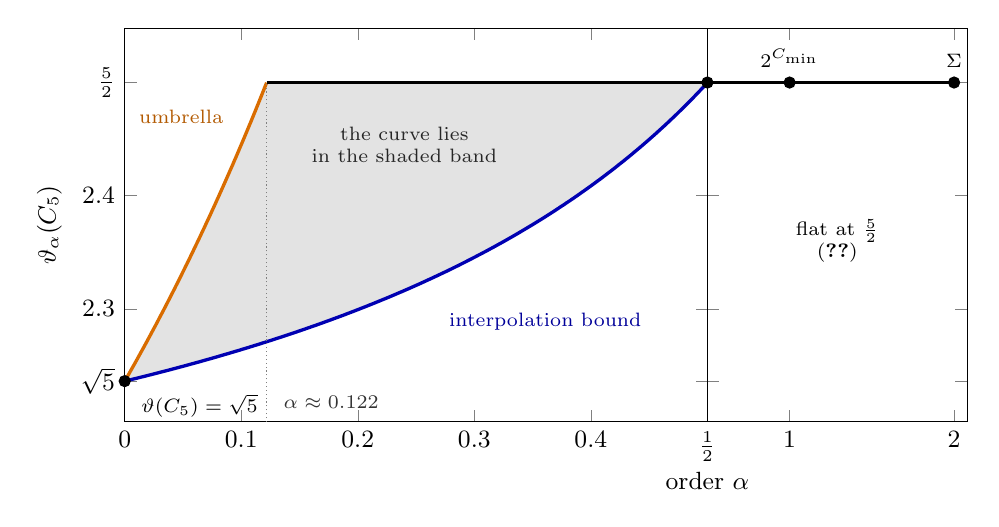
\begin{tikzpicture}
\begin{groupplot}[
  group style={group size=2 by 1, horizontal sep=0pt, yticklabels at=edge left},
  scale only axis, height=5.0cm,
  ymin=2.200, ymax=2.548,
  ytick={2.2360679775,2.3,2.4,2.5},
  yticklabels={$\sqrt5$,$2.3$,$2.4$,$\tfrac52$},
  tick label style={font=\small},
  set layers,
  clip=false,
]
\nextgroupplot[width=7.4cm, xmin=0, xmax=0.5,
  xtick={0,0.1,0.2,0.3,0.4,0.5},
  xticklabels={$0$,$0.1$,$0.2$,$0.3$,$0.4$,$\tfrac12$},
  ylabel={$\vt_\alpha(C_5)$}, ylabel style={font=\small}]
  \addplot[name path=up, draw=none, domain=0:0.5, samples=240]
     {min(2.5, 5^(1/(2-2*x)))};
  \addplot[name path=lo, draw=none, domain=0:0.5, samples=240]
     {sqrt(5)*(sqrt(5)/2)^(x/(1-x))};
  \addplot[gray!22, on layer=pre main] fill between[of=up and lo];
  \addplot[very thick, orange!85!black, domain=0:0.1217646, samples=200]
     {5^(1/(2-2*x))};
  \addplot[very thick, black, domain=0.1217646:0.5] {2.5};
  \addplot[very thick, blue!70!black, domain=0:0.5, samples=240]
     {sqrt(5)*(sqrt(5)/2)^(x/(1-x))};
  \draw[densely dotted, gray] (axis cs:0.1217646,2.200) -- (axis cs:0.1217646,2.5);
  \node[font=\scriptsize, gray!40!black, anchor=south west]
     at (axis cs:0.128,2.203) {$\alpha\approx0.122$};
  \addplot[only marks, mark=*, mark size=2pt] coordinates {(0,2.2360679775) (0.5,2.5)};
  \node[font=\scriptsize, anchor=north west] at (axis cs:0.006,2.233) {$\vt(C_5)=\sqrt5$};
  \node[font=\scriptsize, orange!70!black, anchor=west]
     at (axis cs:0.004,2.47) {umbrella};
  \node[font=\scriptsize, blue!60!black, anchor=north west]
     at (axis cs:0.27,2.305) {interpolation bound};
  \node[font=\scriptsize, gray!30!black, align=center]
     at (axis cs:0.24,2.445) {the curve lies\\in the shaded band};
\nextgroupplot[width=3.3cm, xmin=0.5, xmax=2.08,
  xtick={1,2}, xticklabels={$1$,$2$}]
  \addplot[very thick, black, domain=0.5:2] {2.5};
  \addplot[only marks, mark=*, mark size=2pt] coordinates {(1,2.5) (2,2.5)};
  \node[font=\scriptsize, anchor=south] at (axis cs:1,2.505) {$2^{\Cmin}$};
  \node[font=\scriptsize, anchor=south] at (axis cs:2,2.505) {$\Sigma$};
  \node[font=\scriptsize, align=center] at (axis cs:1.29,2.36)
     {flat at $\tfrac52$\\(\cref{thm:pentagon-half})};
\end{groupplot}
\node[font=\small] at ($(group c1r1.south east)+(0,-0.75)$) {order $\alpha$};
\end{tikzpicture}
\caption{What is known about $\alpha\mapsto\vt_\alpha(C_5)$.  The
horizontal scale changes at $\alpha=\tfrac12$.  On $[\tfrac12,2]$ the curve is
exactly $\tfrac52$, which gives $\Cmin(C_5)=\log_2\tfrac52$ and
$\Sigma(C_5)=\tfrac52$.  On $[0,\tfrac12]$ it is continuous and nondecreasing
and lies between the interpolation lower bound (blue) and the minimum of
$\tfrac52$ and the Lov\'asz-umbrella bound (orange).  The umbrella bound is
better than $\tfrac52$ only for $\alpha<1-\ln5/(2\ln\frac52)\approx0.122$.
Continuity and the endpoint values $\sqrt5$ and $\tfrac52$ force the curve
through every value in between.}
\label{fig:pentagon-curve}
\end{figure}

The pentagon cannot tell order one from order two.  A different graph can.

\begin{mainthm}[order one is not order two]\label{thm:C}
There is a graph $G_{32}$ on $32$ vertices, built from the Mermin--Peres
magic square, such that
\[
 2^{\Cmin(G_{32})}\ \le\ 6.186983\ldots\ <\ 6.194232\ldots\ \le\ \Sigma(G_{32}).
\]
Both outer bounds are certified by exact rational data.  In particular
$\vt_1\ne\vt_2$.
\end{mainthm}

\subsection{A taste of the method: the pentagon in one inequality}
\label{sec:taste}

The pentagon conjecture has a proof short enough to give here in full.  Label
$C_5$ by $\mathbb Z_5$ with $i\sim i\pm1$.  In a representation of the
pentagon, non-neighbours get orthogonal projections: $P_iP_{i+2}=0$ for all
$i$.  At order $\alpha=\frac12$, the formula of \cref{sec:compressions} for
$\vt_\alpha$ becomes
\[
 \frac{1}{\vt_{1/2}(G)}
 =\sup_{(P_x),\,\sigma}\ \min_x\ \nrm{P_x\sigma^{1/2}P_x}_2^2 ,
\]
the supremum running over representations $(P_x)$ of $G$ and faithful states
$\sigma$.  Now the one inequality we need: for every representation of $C_5$
and every matrix $X$,
\begin{equation}\label{eq:hs-intro}
 \sum_{i\in\mathbb Z_5}\nrm{P_iXP_i}_2^2\ \le\ 2\,\nrm{X}_2^2 .
\end{equation}
The reason is local.  The two neighbours $i-1$ and $i+1$ of a vertex are not
adjacent to each other, so $P_{i-1}+P_{i+1}$ is again a projection.  Seen from
inside $P_i$, the sum of all five projections is therefore at most twice the
identity (\cref{lem:hs}).  Put $X=\sigma^{1/2}$.  The right side of~\eqref{eq:hs-intro}
is $2\Tr\sigma=2$, so some vertex has $\nrm{P_i\sigma^{1/2}P_i}_2^2\le2/5$,
and $\vt_{1/2}(C_5)\ge5/2$.  Since $\vt_\alpha$ increases with $\alpha$, the
same bound holds for $\vt_1=2^{\Cmin}$ and for $\vt_2=\Sigma$.

The matching upper bound is the obvious classical channel: input $i$ produces a
uniformly random element of $\{i,i+1\}$.  Its Holevo capacity is
$\log_25-1=\log_2\frac52$, and $T=\frac12 I$ dominates every output with
$\Tr T=\frac52$.  Duan and Winter's chain~\eqref{eq:dw-chain} squeezes $\SNS$
in between, and $\alpha^*(C_5)=\frac52$ is classical.  That is the whole proof.

\subsection{What is new}\label{sec:new}

\paragraph{New points in the entanglement-assisted spectrum.}
To our knowledge, the parameters $\vt_\alpha$ with $\alpha>0$ are the first
elements of $\Xs$ other than $\vt$.  \Cref{thm:B} settles Li and Zuiddam's
``only point'' question in the negative.  It says nothing about whether $\vt$
is the \emph{least} point.  Every $\vt_\alpha$ dominates $\vt$, so the bound
$\Theta_*\le\vt$ is not improved and the conjecture $\Theta_*=\vt$ is
untouched.

\paragraph{Multiplicativity for joint representations.}
Duan and Winter proved that $\Sigma$ is multiplicative for two \emph{fixed}
cq-graphs \cite{DuanWinter2016}.  In our language, that is the case of
\cref{thm:product} in which the representation of $G\boxt H$ is a tensor
product.  \Cref{thm:product} drops that assumption, at every order in
$[0,2]$.  At the two lower endpoints this recovers known results: order zero
is Lov\'asz's multiplicativity of $\vt$ \cite{Lovasz1979}, and order one is
Duan and Winter's additivity of $\Cmin$ under the strong product
\cite[Lemma~23]{DuanWinter2016}.  Every order in $(0,1)\cup(1,2]$ is new, and
order two is the one with an operational consequence.  There it gives a
single-letter formula,
\[
 \SNS(G)=\log_2\Sigma(G),
\]
for the optimal asymptotic no-signalling simulation rate among channels with
confusability graph $G$.  Duan and Winter single out asymptotic simulation
with no-signalling assistance as an important open problem.  At the level of
confusability graphs, this reduces it to a one-shot problem.

\paragraph{The Duan--Winter chain, link by link.}
With~\eqref{eq:endpoints-intro} in hand, every link of~\eqref{eq:dw-chain}
can now be decided (\cref{fig:chain}).  Duan and Winter showed that the last
link can be strict.  They conjectured that the first is strict on the
pentagon, which is the corollary above.  They left open whether either of the
two middle links can be strict.  The third link is always an equality
(\cref{thm:A} at order two).  The second can be strict (\cref{thm:C}).

\paragraph{One curve instead of three numbers.}
Duan and Winter already wrote $\log_2\Sigma$ as a conditional min-entropy,
which is a max-relative-entropy radius.  What seems to be new is that, once
one minimizes over states supported in a fixed projection, this radius
coincides with the \emph{Petz} radius of order two.  All three quantities then
sit on a single monotone curve.  Above order one the curve is also the same
for the sandwiched R\'enyi divergences: the sandwiched radius of order
$\beta\ge1$ equals $\vt_{2-1/\beta}$ (\cref{prop:sandwiched}), so nothing
depends on which quantum R\'enyi divergence one prefers there.  The picture has a useful by-product: every
$\vt_\alpha$ is squeezed between $\vt$ and $\alpha^*$ by flat witnesses
(\cref{prop:endpoints}).  So the family collapses to a single value on graphs
with $\vt=\alpha^*$, perfect graphs among them, and it can only separate
points on graphs with $\vt<\alpha^*$.

\begin{figure}[t]
\centering
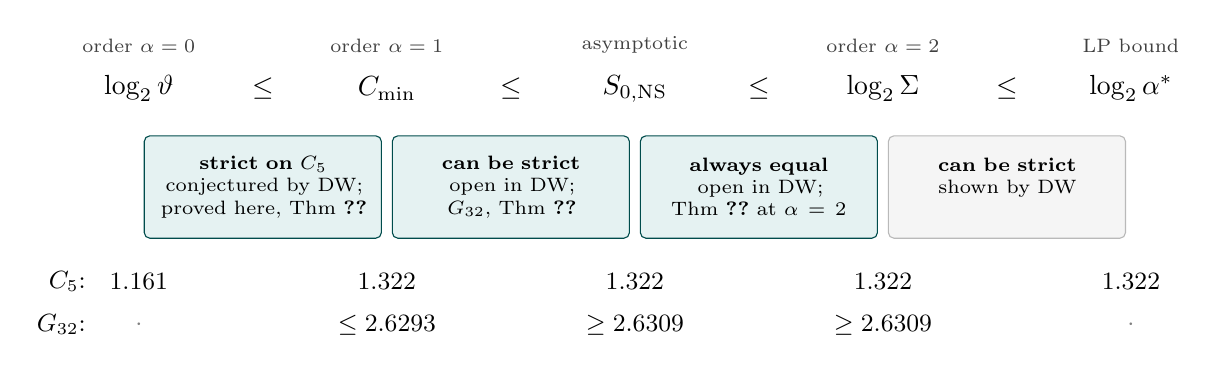
\begin{tikzpicture}[
  q/.style={font=\normalsize, inner sep=2pt, minimum height=0.6cm},
  ord/.style={font=\scriptsize, gray!50!black},
  st/.style={draw, rounded corners=2pt, align=center, font=\scriptsize,
             text width=2.8cm, inner sep=3pt, minimum height=1.3cm},
  new/.style={st, fill=teal!10, draw=teal!60!black},
  old/.style={st, fill=gray!8, draw=gray!55},
  val/.style={font=\small},
]
\def\dx{3.15}
\node[q] (a) at (0,0)      {$\log_2\vt$};
\node[q] (b) at (\dx,0)    {$\Cmin$};
\node[q] (c) at (2*\dx,0)  {$\SNS$};
\node[q] (d) at (3*\dx,0)  {$\log_2\Sigma$};
\node[q] (e) at (4*\dx,0)  {$\log_2\alpha^*$};
\foreach \u/\v in {a/b,b/c,c/d,d/e} \node at ($(\u)!0.5!(\v)$) {$\le$};
\node[ord] at (0,0.55)     {order $\alpha=0$};
\node[ord] at (\dx,0.55)   {order $\alpha=1$};
\node[ord] at (2*\dx,0.55) {asymptotic};
\node[ord] at (3*\dx,0.55) {order $\alpha=2$};
\node[ord] at (4*\dx,0.55) {LP bound};
\node[new] at ($(a)!0.5!(b)+(0,-1.25)$)
  {\textbf{strict on $C_5$}\\ conjectured by DW;\\ proved here, Thm~\ref{thm:B}};
\node[new] at ($(b)!0.5!(c)+(0,-1.25)$)
  {\textbf{can be strict}\\ open in DW;\\ $G_{32}$, Thm~\ref{thm:C}};
\node[new] at ($(c)!0.5!(d)+(0,-1.25)$)
  {\textbf{always equal}\\ open in DW;\\ Thm~\ref{thm:A} at $\alpha=2$};
\node[old] at ($(d)!0.5!(e)+(0,-1.25)$)
  {\textbf{can be strict}\\ shown by DW\\ \phantom{x}};
\node[font=\small, anchor=east] at (-0.55,-2.45) {$C_5$:};
\node[val] at (0,-2.45)      {$1.161$};
\node[val] at (\dx,-2.45)    {$1.322$};
\node[val] at (2*\dx,-2.45)  {$1.322$};
\node[val] at (3*\dx,-2.45)  {$1.322$};
\node[val] at (4*\dx,-2.45)  {$1.322$};
\node[font=\small, anchor=east] at (-0.55,-3.0) {$G_{32}$:};
\node[val, gray] at (0,-3.0)     {$\cdot$};
\node[val] at (\dx,-3.0)   {$\le2.6293$};
\node[val] at (2*\dx,-3.0) {$\ge2.6309$};
\node[val] at (3*\dx,-3.0) {$\ge2.6309$};
\node[val, gray] at (4*\dx,-3.0) {$\cdot$};
\end{tikzpicture}
\caption{The Duan--Winter chain~\eqref{eq:dw-chain} after this paper.  The
three quantities in the first four columns that carry an order are the points
$\alpha=0,1,2$ of one curve.  Shaded boxes record the status of each link;
teal marks what is new here.  The bottom rows give values in bits (dots are
values we do not need).}
\label{fig:chain}
\end{figure}

\subsection{Related work}

Dalai showed that the Lov\'asz bound and the sphere-packing bound for
classical--quantum channels are both information radii of Csisz\'ar type
built from R\'enyi divergences \cite{Dalai2013}.  Our order-zero endpoint is an
object of the same kind, and the family $\vt_\alpha$ continues it to positive
order at the level of graphs.  As explained above, Duan and Winter's
fixed-cq-graph multiplicativity is the factoring case of our product theorem.
In the ordinary spectrum, continua arise in a different way.  Vrana's
probabilistic refinement makes the ordinary spectrum log-convex in a suitable
sense \cite{Vrana2021}, and so interpolating between two known points produces
new ones.  We do not know whether an analogue holds for $\le_*$.
\Cref{sec:open} explains why, even if it does, at least $\vt_1$ is not such an
interpolation.  For the weaker quantum and commuting-quantum
preorders, Haemers-type parameters give further points
\cite{LiZuiddam2020,GaoGriblingLi2022}.  Their monotonicity under $\le_*$ is
not known.  Finally, Vrana studied which points of the ordinary spectrum
extend to non-commutative graphs \cite{Vrana2022}.  We stay with classical
graphs throughout.

\paragraph{Organization.}
\Cref{sec:setup} fixes conventions.  \Cref{sec:compressions} rewrites
$\vt_\alpha$ in terms of projections and proves the basic properties of the
family.  \Cref{sec:spectral} proves \cref{thm:A}.  \Cref{sec:pentagon}
treats the pentagon and the Duan--Winter chain, and \cref{sec:small}
separates orders one and two.  Open problems are collected in
\cref{sec:open}.  The appendices contain the certificate format and a few
routine proofs.

\section{Setup}\label{sec:setup}

\begin{tcolorbox}[colback=gray!4,colframe=gray!45,boxrule=0.5pt,arc=2pt,
  left=6pt,right=6pt,top=4pt,bottom=4pt,title={\small Conventions},
  fonttitle=\bfseries,coltitle=black,colbacktitle=gray!15]
\small
\begin{itemize}[leftmargin=1.2em,itemsep=2pt,topsep=2pt]
\item Graphs are finite and simple, and they are read as \emph{confusability
graphs}: $x\sim y$ means that inputs $x$ and $y$ may be confused.  We write
$x\simeq y$ for ``$x=y$ or $x\sim y$''.
\item Distinct non-adjacent vertices must be told apart, so they are
represented by \emph{orthogonal} objects.  This is Lov\'asz's original
orientation \cite{Lovasz1979}.  Li and Zuiddam express the same relations
through graph complements.
\item $G\sqcup H$ is the disjoint union and $G\boxt H$ the strong product,
where $(x,y)\simeq(x',y')$ if and only if $x\simeq x'$ and $y\simeq y'$.
$K_1$ is a single vertex, $\overline{K_n}$ is the edgeless graph on $n$
vertices (a noiseless channel with $n$ inputs), and $C_5$ is the pentagon.
\item Logarithms are to base two unless written $\ln$.  Hilbert spaces are
finite-dimensional, of arbitrary dimension.  A state is \emph{faithful} if it
is invertible.  $\Pi_\rho$ is the support projection of $\rho$.
\end{itemize}
\end{tcolorbox}

\subsection{Representations and R\'enyi radii}

\begin{definition}\label{def:representation}
A \emph{representation} of $G$ is a family $(P_x)_{x\in V(G)}$ of nonzero
orthogonal projections on a Hilbert space such that $P_xP_y=0$ whenever
$x\ne y$ are non-adjacent.  A family of states $(\rho_x)$ is
\emph{compatible with} $G$ if its supports form a representation.
\end{definition}

A compatible family is the same thing as a classical--quantum channel
$x\mapsto\rho_x$ whose confusability graph is contained in $G$: two inputs can
only be confused if they are adjacent.  Extra orthogonality between adjacent
vertices is allowed.  Duan and Winter optimize over the same class of channels.
Readers who prefer channels whose confusability graph is exactly $G$ lose
nothing, because every infimum below is the same for both classes
(\cref{lem:exact-graph}).

For a state $\rho$ and a faithful state $\sigma$, the Petz--R\'enyi
divergence of order $\alpha\in(0,1)\cup(1,2]$ is
\[
 D_\alpha(\rho\Vert\sigma)=\frac{1}{\alpha-1}\log\Tr\rho^\alpha\sigma^{1-\alpha}.
\]
At $\alpha=1$ it is the relative entropy $D(\rho\Vert\sigma)$, and at
$\alpha=0$ it is $D_0(\rho\Vert\sigma)=-\log\Tr\Pi_\rho\sigma$.  We use four
standard facts \cite{Petz1986,Tomamichel2016}.  The divergence is
nonnegative and vanishes at $\rho=\sigma$.  It is additive under tensor
products.  It is nondecreasing in $\alpha$.  And it satisfies data processing
for every $\alpha\in[0,2]$.

\begin{definition}\label{def:theta-alpha}
For a graph $G$ and $\alpha\in[0,2]$, define $\vt_\alpha(G)$ by
\begin{equation}\label{eq:def-parameter}
 \log\vt_\alpha(G)
 =\inf\Bigl\{\max_{x}D_\alpha(\rho_x\Vert\sigma)\ :\
   (\rho_x)\text{ compatible with }G,\ \sigma\text{ faithful}\Bigr\},
\end{equation}
where the states live on a common Hilbert space of any finite dimension.  For
the empty graph we set $\vt_\alpha(K_0)=0$.
\end{definition}

Nothing changes if singular centers are allowed with the usual support
conventions: mix a singular center with a little of the maximally mixed state
and let the weight go to zero.

\subsection{The Duan--Winter quantities}\label{sec:dw-quantities}

Duan and Winter attach the following quantities to a graph
\cite{DuanWinter2016}.  The \emph{minimal Holevo capacity} is
\begin{equation}\label{eq:cmin-def}
 \Cmin(G)=\inf_{(\rho_x)\text{ compatible}}\ \max_p
  \Bigl[S\Bigl(\sum_xp_x\rho_x\Bigr)-\sum_xp_xS(\rho_x)\Bigr].
\end{equation}
The \emph{no-signalling simulation cost} is
\begin{equation}\label{eq:sigma-def}
 \Sigma(G)=\inf\bigl\{\Tr T\ :\ T\ge\rho_x\text{ for all }x,\
   (\rho_x)\text{ compatible}\bigr\}.
\end{equation}
Duan and Winter show that $\min\{\Tr T:T\ge\rho_x\ \forall x\}$ is the real
SDP value governing exact simulation of the channel $x\mapsto\rho_x$ with
no-signalling assistance.  For a fixed channel, the literal one-shot
noiseless message alphabet has size equal to the ceiling of this SDP value;
the ceiling disappears after division by block length.  At graph level,
$\Sigma(G)$ is an infimum over compatible channels and need not be attained.
Thus $\log\Sigma(G)$ is the infimum of the corresponding single-letter SDP
costs.  Tensoring witnesses shows that $\Sigma$ is
submultiplicative under $\boxt$, so the regularization
\[
 \SNS(G)=\lim_{n\to\infty}\frac1n\log\Sigma(G^{\boxt n})
\]
exists.  This is Duan and Winter's graph-level asymptotic simulation cost.
Finally, $\alpha^*(G)$ is the fractional packing number: the largest
$\sum_xv_x$ over $v\ge0$ with $\sum_{x\in C}v_x\le1$ for every clique $C$.  By
LP duality it is also the smallest $\sum_Cw_C$ over $w\ge0$ with
$\sum_{C\ni x}w_C\ge1$ for every vertex $x$.

\subsection{The entanglement-assisted spectrum}

We use the entanglement-assisted cohomomorphism preorder of Li and Zuiddam
\cite{LiZuiddam2020}, which comes from the entanglement-assisted
homomorphisms of Cubitt et al.~\cite{CMRSSW2014}.  In confusability language,
$G\le_*H$ means that there are a state $\omega$ and positive semidefinite
operators $\omega_g^h$ ($g\in V(G)$, $h\in V(H)$) with
\begin{align}
 \sum_{h\in V(H)}\omega_g^h&=\omega\quad\text{for every }g,\label{eq:ea-sum}\\
 \omega_g^h\,\omega_{g'}^{h'}&=0\quad\text{whenever $g\ne g'$ are non-adjacent
 in $G$ and $h\simeq h'$ in $H$.}\label{eq:ea-orth}
\end{align}
Here is the operational picture.  Alice and Bob share a pure entangled state,
and $\omega$ is Bob's half of it.  To send $g$, Alice measures her half with a
measurement that depends on $g$, obtains an outcome $h$, and sends $h$ through
a channel with confusability graph $H$.  Her measurement steers Bob's half to
$\omega_g^h$ (unnormalized), and~\eqref{eq:ea-sum} says that Bob's marginal
does not depend on $g$.  Suppose $g$ and $g'$ must be told apart but the
channel might confuse $h$ with $h'$.  Then~\eqref{eq:ea-orth} lets Bob tell
them apart anyway, by measuring his own half.  So $G\le_*H$ says that, with
entanglement, one use of an $H$-channel does everything one use of a
$G$-channel does.  For example, $\overline{K_n}\le_*G$ says that $n$ messages
can be sent without error over one use of $G$.

\begin{definition}
The \emph{entanglement-assisted asymptotic spectrum} $\Xs$ is the set of maps
$\phi$ from finite graphs to $[0,\infty)$ such that
\[
 \phi(G\sqcup H)=\phi(G)+\phi(H),\quad
 \phi(G\boxt H)=\phi(G)\phi(H),\quad
 \phi(K_1)=1,\quad
 G\le_*H\Rightarrow\phi(G)\le\phi(H).
\]
\end{definition}

Li and Zuiddam show that $\Theta_*(G)=\min_{\phi\in\Xs}\phi(G)$, and that
$\vt\in\Xs$ \cite{LiZuiddam2020}.

\section{Power compressions and the shape of the family}
\label{sec:compressions}

The definition~\eqref{eq:def-parameter} optimizes over states.  It is much
easier to work with projections, and the tool for this is the following
compression.

\subsection{From states to projections}

Let $P\ne0$ be a projection, let $\sigma$ be faithful, and let
$s\in[-1,1]$.  On $\ran P$ define
\[
 K_s(\sigma,P)=
 \begin{cases}(P\sigma^sP)^{1/s}, & s\ne0,\\ \exp\bigl(P(\ln\sigma)P\bigr), & s=0,\end{cases}
 \qquad Z_s(\sigma,P)=\Tr K_s(\sigma,P),
\]
extended by zero off $\ran P$.  We call $K_s$ the \emph{power compression} of
$\sigma$ to $P$ and $Z_s$ its \emph{weight}.  Four values of $s$ recur.
$Z_1=\Tr P\sigma$ is the plain weight.  $Z_{1/2}=\nrm{P\sigma^{1/2}P}_2^2$ is
a Hilbert--Schmidt weight.  $Z_0$ is a Gibbs weight.  And
$Z_{-1}=\Tr(P\sigma^{-1}P)^{-1}$ is the trace of the \emph{shorted operator}
$\sigma_{/P}$, the largest positive operator below $\sigma$ with range in
$\ran P$ \cite{AndersonTrapp1975}.  All the weights are homogeneous of degree
one: $K_s(c\sigma,P)=c\,K_s(\sigma,P)$ for $c>0$.

\begin{proposition}[supported minimization]\label{prop:supported}
Let $0\le\alpha\le2$ and $s=1-\alpha$.  Then
\[
 \min_{\rho:\ \supp\rho\subseteq\ran P}D_\alpha(\rho\Vert\sigma)
 =-\log Z_s(\sigma,P),
\]
and the minimum is attained at $\rho=K_s(\sigma,P)/Z_s(\sigma,P)$.
\end{proposition}

\begin{proof}
For $\rho$ supported in $P$ we have
$\Tr\rho^\alpha\sigma^s=\Tr\rho^\alpha A$ with $A=P\sigma^sP$, and
$Z_s=\Tr A^{1/s}$ when $s\ne0$.

\emph{Case $0<\alpha<1$.}  Here $s\in(0,1)$.  H\"older's inequality for
Schatten norms gives
$\Tr\rho^\alpha A\le\nrm{\rho^\alpha}_{1/\alpha}\nrm{A}_{1/s}
=(\Tr A^{1/s})^s$.  Since $\alpha-1<0$, this becomes
$D_\alpha(\rho\Vert\sigma)\ge\frac{s}{\alpha-1}\log Z_s=-\log Z_s$, with
equality at $\rho\propto A^{1/s}$.

\emph{Case $1<\alpha\le2$.}  Now $s\in[-1,0)$ and $A$ is positive definite on
$\ran P$.  Write $A=\sum_ka_k\proj{e_k}$ and $q_k=\bra{e_k}\rho\ket{e_k}$, a
probability vector.  Convexity of $t\mapsto t^\alpha$ gives
$\bra{e_k}\rho^\alpha\ket{e_k}\ge q_k^\alpha$, so
$\Tr\rho^\alpha A\ge\sum_ka_kq_k^\alpha$.  By H\"older,
\[
 1=\sum_k\bigl(a_k^{1/\alpha}q_k\bigr)a_k^{-1/\alpha}
 \le\Bigl(\sum_ka_kq_k^\alpha\Bigr)^{1/\alpha}
    \Bigl(\sum_ka_k^{1/s}\Bigr)^{(\alpha-1)/\alpha},
\]
using $-1/(\alpha-1)=1/s$.  Hence
$\Tr\rho^\alpha A\ge(\sum_ka_k^{1/s})^{s}=Z_s^s$, and dividing the logarithm
by $\alpha-1>0$ gives $D_\alpha\ge-\log Z_s$.  Equality holds when $\rho$ is
diagonal in $(e_k)$ with $q_k\propto a_k^{1/s}$, that is, at
$\rho\propto A^{1/s}$.

\emph{Case $\alpha=1$.}  On $\ran P$ we have
$\ln K_0=P(\ln\sigma)P$, so $\Tr\rho\ln\sigma=\Tr\rho\ln(K_0/Z_0)+\ln Z_0$ and
$D(\rho\Vert\sigma)=D(\rho\Vert K_0/Z_0)-\log Z_0\ge-\log Z_0$.

\emph{Case $\alpha=0$.}  $\Tr\Pi_\rho\sigma\le\Tr P\sigma=Z_1$, with equality
whenever $\rho$ has full support in $\ran P$.
\end{proof}

The minimizers for different vertices have the supports we prescribe, so they
form a compatible family whenever the projections form a representation.
Conversely, the supports of any compatible family form a representation.  This
proves the projection formula:
\begin{equation}\label{eq:projection-formula}
 \frac1{\vt_\alpha(G)}
 =\sup_{(P_x),\,\sigma}\ \min_{x\in V(G)}Z_{1-\alpha}(\sigma,P_x),
\end{equation}
with the supremum over representations of $G$ and faithful states $\sigma$ on
the same space.

\subsection{Endpoints, flat witnesses and a sandwich}

Some witnesses have the same radius at every order.  Call a pair
$(\rho,\sigma)$ \emph{flat} if $\sigma$ commutes with a projection $\Pi$ and
$\rho=\Pi\sigma/\Tr\Pi\sigma$.

\begin{lemma}[flat witnesses]\label{lem:flat}
If $(\rho,\sigma)$ is flat, then $D_\alpha(\rho\Vert\sigma)=-\log\Tr\Pi\sigma$
for every $\alpha\in[0,2]$.
\end{lemma}

\begin{proof}
With $c=\Tr\Pi\sigma$ we get
$\Tr\rho^\alpha\sigma^{1-\alpha}=c^{-\alpha}\Tr\Pi\sigma=c^{1-\alpha}$, which
gives the claim for $\alpha\ne0,1$.  The two remaining orders are direct.
\end{proof}

\begin{proposition}\label{prop:endpoints}
For every graph $G$:
\begin{enumerate}[label=\textup{(\roman*)},itemsep=1pt]
\item $\vt_0(G)=\vt(G)$, $\vt_1(G)=2^{\Cmin(G)}$ and $\vt_2(G)=\Sigma(G)$;
\item $\alpha\mapsto\vt_\alpha(G)$ is nondecreasing on $[0,2]$;
\item $\vt(G)\le\vt_\alpha(G)\le\alpha^*(G)$ for every $\alpha\in[0,2]$.
\end{enumerate}
\end{proposition}

\begin{proof}
(i) \emph{Order zero.}  By~\eqref{eq:projection-formula},
$1/\vt_0(G)=\sup\min_x\Tr P_x\sigma$.  Lov\'asz's handle form reads
$1/\vt(G)=\sup\min_x|\langle c,u_x\rangle|^2$ over orthonormal
representations $(u_x)$ of $G$ and unit vectors $c$ \cite{Lovasz1979}.  A
vector representation is a projection representation with $P_x=\proj{u_x}$,
and a faithful approximation of $\proj c$ gives $\vt_0\le\vt$.  Conversely,
purify $\sigma$ to a unit vector $c\in\cH\otimes\cH'$ and put
$u_x\propto(P_x\otimes I)c$.  Non-adjacent vertices get orthogonal vectors,
and $|\langle c,u_x\rangle|^2=\Tr P_x\sigma$, so $\vt\le\vt_0$.

\emph{Order one.}  For each compatible family, the Holevo capacity equals the
relative-entropy radius $\min_\sigma\max_xD(\rho_x\Vert\sigma)$
\cite{SchumacherWestmoreland2001}.  Taking the infimum over families gives
$\vt_1=2^{\Cmin}$.

\emph{Order two.}  By~\eqref{eq:projection-formula},
$1/\vt_2=\sup\min_x\Tr\sigma_{/P_x}$.  Given a compatible family and $T\ge\rho_x$
with $t=\Tr T$, put $\sigma=T/t$, regularized if needed.  Each $\rho_x/t$ lies
below $\sigma$ with range in $\ran P_x$, so $\Tr\sigma_{/P_x}\ge1/t$.  Hence
$\vt_2\le\Sigma$.  Conversely, if $\Tr\sigma_{/P_x}\ge c$ for all $x$, the
states $\rho_x=\sigma_{/P_x}/\Tr\sigma_{/P_x}$ are compatible and all lie below
$T=\sigma/c$, whose trace is $1/c$.  Hence $\Sigma\le\vt_2$.

(ii) $D_\alpha$ is nondecreasing in $\alpha$ for each pair of states, and
infima preserve this.

(iii) The lower bound follows from (i) and (ii).  For the upper bound take a
fractional clique cover $w$ with $\sum_Cw_C=\alpha^*(G)$, and work on the
space spanned by orthonormal vectors $\ket C$, one for each clique with
$w_C>0$.  Put $\sigma=\sum_Cw_C\proj C/\alpha^*(G)$ and let $\Pi_x$ project
onto the cliques containing $x$.  Non-adjacent vertices share no clique, so the
flat states $\rho_x=\Pi_x\sigma/\Tr\Pi_x\sigma$ are compatible.  By
\cref{lem:flat} their radius at every order is
$\max_x\log\bigl(\alpha^*(G)/\sum_{C\ni x}w_C\bigr)\le\log\alpha^*(G)$.
\end{proof}

Two consequences are worth stating.  First, if $\vt(G)=\alpha^*(G)$, the
whole family collapses on $G$.  This happens for every perfect graph.  Second,
if some flat witness is optimal for $\vt_1(G)$, then $\vt_1(G)=\vt_2(G)$,
because the flat radius does not depend on the order.  On the pentagon, this
is exactly what happens (\cref{sec:pentagon}).

\subsection{Continuity}

\begin{proposition}\label{prop:continuity}
For every graph $G$, the map $\alpha\mapsto\vt_\alpha(G)$ is continuous on
$[0,1)$.
\end{proposition}

Right continuity comes from fixing a near-optimal witness.  Left continuity
comes from a comparison $D_\alpha\le\frac{\alpha(1-\beta)}{\beta(1-\alpha)}D_\beta$
for $\beta<\alpha<1$, whose constant does not depend on the states or the
dimension.  The details are in \cref{app:continuity}.

\subsection{Sandwiched radii give the same curve}\label{sec:sandwiched}

The Petz divergence is not the only quantum R\'enyi divergence.  For
$\beta\in(1,\infty)$ the \emph{sandwiched} R\'enyi divergence
\cite{MDSFT2013,WWY2014} is
\[
 \widetilde D_\beta(\rho\Vert\sigma)
 =\frac1{\beta-1}\log\Tr\Bigl(\sigma^{\frac{1-\beta}{2\beta}}\,\rho\,
   \sigma^{\frac{1-\beta}{2\beta}}\Bigr)^{\beta},
\]
with the relative entropy $\widetilde D_1=D$ and the max-relative entropy
$\widetilde D_\infty(\rho\Vert\sigma)=\log\min\{\lambda:\rho\le\lambda\sigma\}$
at the two ends.  Define $\widetilde\vt_\beta(G)$
by~\eqref{eq:def-parameter} with $\widetilde D_\beta$ in place of $D_\alpha$.
Above order one, this gives nothing new.

\begin{proposition}[sandwiched radii]\label{prop:sandwiched}
For every graph $G$ and every $\beta\in[1,\infty]$,
\[
 \widetilde\vt_\beta(G)=\vt_{2-1/\beta}(G),
\]
with $2-1/\infty=2$.  In particular $\widetilde\vt_1=2^{\Cmin}$ and
$\widetilde\vt_\infty=\Sigma$.
\end{proposition}

\begin{proof}
Put $\theta=(\beta-1)/\beta\in[0,1]$, so that $s=-\theta$ is the parameter of
the Petz order $\alpha=1-s=2-1/\beta$.  The argument leading
to~\eqref{eq:projection-formula} applies verbatim once we know the supported
minimum: for a projection $P\ne0$ and a faithful state $\sigma$,
\begin{equation}\label{eq:sandwiched-supported}
 \min_{\rho:\ \supp\rho\subseteq\ran P}\widetilde D_\beta(\rho\Vert\sigma)
 =-\log Z_{-\theta}(\sigma,P).
\end{equation}
At $\beta=1$ this is \cref{prop:supported} at order one.  At $\beta=\infty$,
the condition $\rho\le\lambda\sigma$ for a state supported in $\ran P$ says that
$\rho/\lambda$ lies below $\sigma$ with range in $\ran P$, so
$1/\lambda\le\Tr\sigma_{/P}=Z_{-1}(\sigma,P)$, with equality at
$\rho=\sigma_{/P}/\Tr\sigma_{/P}$.

Now let $1<\beta<\infty$.  Put $A=P\sigma^{-\theta}P$, which is positive
definite on $\ran P$, and $X=A^{1/2}\rho A^{1/2}$.  The operator
$\sigma^{-\theta/2}\rho\,\sigma^{-\theta/2}$ has the same nonzero eigenvalues
as $\rho^{1/2}\sigma^{-\theta}\rho^{1/2}=\rho^{1/2}A\rho^{1/2}$, and hence as
$X$, so the sandwiched moment is $\Tr X^\beta$.  Since
$\Tr A^{-1}X=\Tr\rho=1$, H\"older's inequality with the conjugate exponents
$\beta$ and $\beta/(\beta-1)=1/\theta$ gives
\[
 1\le\nrm X_\beta\,\nrm{A^{-1}}_{1/\theta}
 =\bigl(\Tr X^\beta\bigr)^{1/\beta}\bigl(\Tr A^{-1/\theta}\bigr)^{\theta}.
\]
Here $A^{-1/\theta}=(P\sigma^{-\theta}P)^{1/(-\theta)}=K_{-\theta}(\sigma,P)$,
so $\Tr X^\beta\ge Z_{-\theta}(\sigma,P)^{-(\beta-1)}$, which is the lower bound
in~\eqref{eq:sandwiched-supported}.  At $\rho=K_{-\theta}/Z_{-\theta}$ we get
$X\propto A^{1-1/\theta}$, so $X^\beta\propto A^{-1/\theta}=(A^{-1})^{1/\theta}$,
which is the equality case of H\"older's inequality.
\end{proof}

So above order one the curve does not depend on which of the two standard
quantum R\'enyi divergences is used: the sandwiched radii of orders
$\beta\in[1,\infty]$ trace exactly the Petz curve on $[1,2]$.  By
\cref{thm:A}, every $\widetilde\vt_\beta$ with $\beta\ge1$ is therefore a point
of $\Xs$ as well.  What happens below order one is discussed in
\cref{sec:open}.

\subsection{The tower identity}

The key algebraic fact is that compressing in two steps is the same as
compressing in one.

\begin{lemma}[tower identity]\label{lem:tower}
Let $P\le Q$ be projections and $s\in[-1,1]$.  Compute the outer compression
below inside $\ran Q$, where $K_s(\sigma,Q)$ is faithful.  Then
\[
 K_s\bigl(K_s(\sigma,Q),P\bigr)=K_s(\sigma,P).
\]
Consequently, if $z=Z_s(\sigma,Q)$, then
$Z_s\bigl(K_s(\sigma,Q)/z,\,P\bigr)=Z_s(\sigma,P)/z$.
\end{lemma}

\begin{proof}
For $s\ne0$, the $s$-th power of $K_s(\sigma,Q)$ inside $\ran Q$ is
$Q\sigma^sQ$, and compressing further to $P\le Q$ gives $P\sigma^sP$.  For
$s=0$ the same computation works with logarithms.  The second statement
follows from homogeneity.
\end{proof}

\section{Every order up to two is a spectral point}\label{sec:spectral}

We need four properties: normalization, additivity under $\sqcup$,
multiplicativity under $\boxt$, and monotonicity under $\le_*$.
Normalization is immediate.  On $K_1$ the divergence is nonnegative and
vanishes at $\rho=\sigma$, so $\vt_\alpha(K_1)=1$.  The product is the heart
of the matter, so we start there.

\subsection{Products}

\begin{figure}[t]
\centering
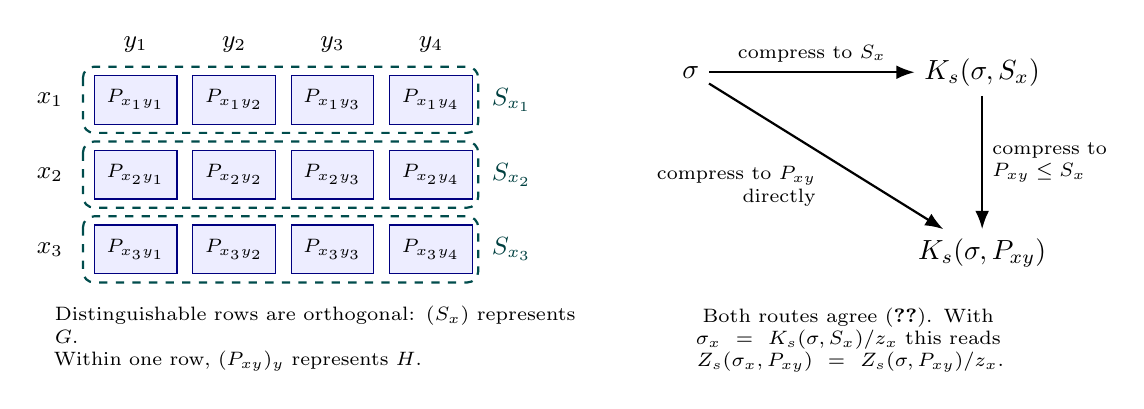
\begin{tikzpicture}[
  cell/.style={draw=blue!50!black, fill=blue!7, minimum width=1.05cm,
               minimum height=0.62cm, font=\scriptsize, inner sep=0pt},
  >=Latex]
\foreach \i in {1,2,3} {
  \foreach \j in {1,2,3,4} {
    \node[cell] (c\i\j) at (1.25*\j, -0.95*\i) {$P_{x_{\i}y_{\j}}$};
  }
  \node[font=\small, anchor=east] at (0.45,-0.95*\i) {$x_{\i}$};
  \draw[rounded corners=4pt, dashed, thick, teal!60!black]
     (0.58,-0.95*\i+0.42) rectangle (5.6,-0.95*\i-0.42);
  \node[font=\small, teal!50!black, anchor=west] at (5.65,-0.95*\i) {$S_{x_{\i}}$};
}
\foreach \j in {1,2,3,4} \node[font=\small] at (1.25*\j,-0.25) {$y_{\j}$};
\node[font=\scriptsize, align=left, anchor=north west, text width=6.8cm]
  at (0.1,-3.45)
  {Distinguishable rows are orthogonal: $(S_x)$ represents $G$.\\
   Within one row, $(P_{xy})_y$ represents $H$.};
\begin{scope}[xshift=8.3cm, yshift=-0.6cm]
  \node (s) at (0,0) {$\sigma$};
  \node (m) at (3.7,0) {$K_s(\sigma,S_x)$};
  \node (p) at (3.7,-2.3) {$K_s(\sigma,P_{xy})$};
  \draw[->, thick] (s) -- node[above, font=\scriptsize] {compress to $S_x$} (m);
  \draw[->, thick] (m) -- node[right, font=\scriptsize, align=left]
       {compress to\\ $P_{xy}\le S_x$} (p);
  \draw[->, thick] (s) -- node[below left, font=\scriptsize, align=right]
       {compress to $P_{xy}$\\ directly} (p);
  \node[font=\scriptsize, align=center, text width=5.4cm] at (2.0,-3.4)
       {Both routes agree (\cref{lem:tower}).  With
        $\sigma_x=K_s(\sigma,S_x)/z_x$ this reads
        $Z_s(\sigma_x,P_{xy})=Z_s(\sigma,P_{xy})/z_x$.};
\end{scope}
\end{tikzpicture}
\caption{The proof of \cref{thm:product}.  Left: a representation of
$G\boxt H$ that need not be a tensor product, organized by rows.  Right: the
tower identity lets each row be analysed with its own reduced center, so the
weight of a cell factors into a $G$-part $z_x$ and an $H$-part.}
\label{fig:product}
\end{figure}

Here is the idea (\cref{fig:product}).  Take any representation $(P_{xy})$ of
$G\boxt H$ and group its projections by the first coordinate.  The ranges in
row $x$ span a subspace, with projection $S_x$.  If $x$ and $x'$ are
distinguishable in $G$, then every cell of row $x$ is distinguishable from
every cell of row $x'$, so $S_x\perp S_{x'}$ and the rows represent $G$.
Inside one row, the cells represent $H$.  All that is missing is a way to
split the weight of a cell into a row part and a within-row part.  The tower
identity does exactly this.

\begin{theorem}[products]\label{thm:product}
For $0\le\alpha\le2$ and all graphs $G,H$,
\[
 \vt_\alpha(G\boxt H)=\vt_\alpha(G)\,\vt_\alpha(H).
\]
\end{theorem}

\begin{proof}
If either graph is empty both sides vanish, so assume both are nonempty and
put $s=1-\alpha$.

For ``$\le$'', take witnesses $(\rho_x),\sigma$ for $G$ and $(\tau_y),\omega$
for $H$.  If $(x,y)$ and $(x',y')$ are distinct and non-adjacent in $G\boxt H$,
then $x,x'$ are distinct and non-adjacent in $G$ or $y,y'$ are in $H$.  In
either case $(\rho_x\otimes\tau_y)(\rho_{x'}\otimes\tau_{y'})=0$.  Since
$D_\alpha$ is additive under tensor products, radii add.

For ``$\ge$'', let $(P_{xy})$ represent $G\boxt H$, let $\sigma$ be faithful,
and suppose $Z_s(\sigma,P_{xy})\ge c>0$ for every pair $(x,y)$.  Let $S_x$ be
the projection onto $\sum_y\ran P_{xy}$, and put $z_x=Z_s(\sigma,S_x)$.

\emph{The rows represent $G$.}  If $x\ne x'$ are non-adjacent in $G$, every
pair $(x,y),(x',y')$ is distinct and non-adjacent in $G\boxt H$, so
$P_{xy}P_{x'y'}=0$ and hence $S_xS_{x'}=0$.

\emph{Each row represents $H$.}  Fix $x$.  If $y\ne y'$ are non-adjacent in
$H$, then $(x,y)$ and $(x,y')$ are non-adjacent, so $(P_{xy})_y$ represents
$H$ on $\ran S_x$.  Use the faithful state $\sigma_x=K_s(\sigma,S_x)/z_x$ on
$\ran S_x$ as center.  By \cref{lem:tower},
$Z_s(\sigma_x,P_{xy})=Z_s(\sigma,P_{xy})/z_x\ge c/z_x$ for every $y$.  The
projection formula~\eqref{eq:projection-formula} for $H$ gives
$c/z_x\le1/\vt_\alpha(H)$, that is, $z_x\ge c\,\vt_\alpha(H)$.

\emph{Combine.}  Apply~\eqref{eq:projection-formula} for $G$ to $(S_x)$ and
$\sigma$: $c\,\vt_\alpha(H)\le\min_xz_x\le1/\vt_\alpha(G)$.  So
$c\le1/(\vt_\alpha(G)\vt_\alpha(H))$ for every admissible $c$, and taking the
supremum gives
\[
 \frac1{\vt_\alpha(G\boxt H)}\le\frac1{\vt_\alpha(G)\,\vt_\alpha(H)} .
 \qedhere
\]
\end{proof}

\begin{remark}\label{rem:single-letter}
At $\alpha=0$ and $\alpha=1$, \cref{thm:product} recovers the multiplicativity
of $\vt$ \cite{Lovasz1979} and Duan and Winter's additivity of $\Cmin$
\cite[Lemma~23]{DuanWinter2016}.  At $\alpha=2$ it says
$\Sigma(G\boxt H)=\Sigma(G)\Sigma(H)$.
Hence $\SNS(G)=\log\Sigma(G)$: regularizing the graph-level SDP value does not
change it.  Their
fixed-cq-graph result \cite{DuanWinter2016} is the special case
$P_{xy}=P_x\otimes Q_y$.
\end{remark}

\subsection{Disjoint unions}

Two small lemmas do the work.  The first rewrites a divergence after
compressing the center.  The second says that the weights of orthogonal blocks
never add up to more than one.

\begin{lemma}[compression identity]\label{lem:compression}
Let $Q\ne0$ be a projection, $s=1-\alpha\in[-1,1]$, and
$\sigma_Q=K_s(\sigma,Q)/Z_s(\sigma,Q)$.  Every state $\rho$ supported in
$\ran Q$ satisfies
\[
 D_\alpha(\rho\Vert\sigma)=D_\alpha(\rho\Vert\sigma_Q)-\log Z_s(\sigma,Q).
\]
\end{lemma}

\begin{proof}
For $\alpha\notin\{0,1\}$, substitute $Q\sigma^sQ=Z_s^s\sigma_Q^s$ into the
Petz moment.  For $\alpha=1$ use $Q(\ln\sigma)Q=\ln\sigma_Q+(\ln Z_0)Q$ on
$\ran Q$, and for $\alpha=0$ use $Q\sigma Q=Z_1\sigma_Q$.
\end{proof}

\begin{lemma}[orthogonal blocks]\label{lem:orthogonal-sum}
If $Q_1,\dots,Q_m$ are mutually orthogonal projections, $\sigma$ is a faithful
state and $s\in[-1,1]$, then $\sum_jZ_s(\sigma,Q_j)\le1$.
\end{lemma}

The proof is a one-line application of Jensen's inequality
(\cref{app:orthogonal-sum}).

\begin{theorem}[disjoint unions]\label{thm:union}
For $0\le\alpha\le2$, $\vt_\alpha(G\sqcup H)=\vt_\alpha(G)+\vt_\alpha(H)$.
\end{theorem}

\begin{proof}
Assume both graphs are nonempty.  For ``$\le$'', put witnesses for $G$ and $H$
with radii at most $\log a$ and $\log b$ on orthogonal summands, and use the
center $(a\sigma_G\oplus b\sigma_H)/(a+b)$.  Compressing this center to the
first summand gives weight $a/(a+b)$ and reduced center $\sigma_G$, so by
\cref{lem:compression} every $G$-state has radius at most
$\log a+\log\frac{a+b}{a}=\log(a+b)$.  The same holds for $H$.

For ``$\ge$'', take a compatible family of $G\sqcup H$ with center $\sigma$
and radius at most $R$.  Let $Q_G$ and $Q_H$ project onto the spans of the
supports of the two subfamilies.  Cross pairs are non-adjacent, so
$Q_GQ_H=0$.  By \cref{lem:compression}, the $G$-states have radius at most
$R+\log Z_s(\sigma,Q_G)$ around $\sigma_{Q_G}$, so
$\vt_\alpha(G)\le2^RZ_s(\sigma,Q_G)$.  Likewise
$\vt_\alpha(H)\le2^RZ_s(\sigma,Q_H)$.  Add the two bounds and apply
\cref{lem:orthogonal-sum}.
\end{proof}

In particular $\vt_\alpha(\overline{K_n})=n$.

\subsection{Entanglement-assisted monotonicity}

The proof follows the protocol described after~\eqref{eq:ea-orth}.  Bob ends
up holding his share of the entanglement together with the channel output.
If $\tau_h$ is the output for $h$, his joint state given $g$ is
$\sum_h\omega_g^h\otimes\tau_h$.  These joint states form a new channel for
$G$, and the only question is whether its radius can be larger than the old
one.  It cannot.  The joint state is a flagged mixture with the flag
discarded, and discarding the flag is data processing.

\begin{lemma}[flagged mixtures]\label{lem:flagged}
Let $\omega_h\ge0$ with $\sum_h\omega_h=\omega$ and $\Tr\omega=1$, let
$\tau_h$ be states and let $\sigma$ be faithful.  If
$D_\alpha(\tau_h\Vert\sigma)\le R$ whenever $\omega_h\ne0$, then for
$0\le\alpha\le2$
\[
 D_\alpha\Bigl(\sum_h\omega_h\otimes\tau_h\ \Big\Vert\ \omega\otimes\sigma\Bigr)\le R .
\]
\end{lemma}

\begin{proof}
Add a classical flag and compare
$\Omega=\sum_h\proj h\otimes\omega_h\otimes\tau_h$ with
$\Omega'=\sum_h\proj h\otimes\omega_h\otimes\sigma$; the support of $\Omega$
lies in that of $\Omega'$.  The Petz moment splits over the flag, and the
$\omega_h$ factors cancel:
\[
 \Tr\Omega^\alpha\Omega'^{1-\alpha}=\sum_hw_h\Tr\tau_h^\alpha\sigma^{1-\alpha},
 \qquad w_h=\Tr\omega_h,\ \ \textstyle\sum_hw_h=1.
\]
For $0<\alpha<1$ each term satisfies
$\Tr\tau_h^\alpha\sigma^{1-\alpha}\ge2^{(\alpha-1)R}$, so the average does too
and $D_\alpha(\Omega\Vert\Omega')\le R$.  For $1<\alpha\le2$ all inequalities
reverse and the conclusion is the same.  At $\alpha=1$ the divergence is the
$w$-average of the $D(\tau_h\Vert\sigma)$, and at $\alpha=0$ we get
$\Tr\Pi_\Omega\Omega'=\sum_hw_h\Tr\Pi_{\tau_h}\sigma\ge2^{-R}$.  Tracing out
the flag maps $\Omega\mapsto\sum_h\omega_h\otimes\tau_h$ and
$\Omega'\mapsto\omega\otimes\sigma$, and Petz divergences of order
$\alpha\in[0,2]$ do not increase under partial traces
\cite{Petz1986,Tomamichel2016}.
\end{proof}

\begin{theorem}[entanglement-assisted monotonicity]\label{thm:ea-mono}
If $G\le_*H$, then $\vt_\alpha(G)\le\vt_\alpha(H)$ for every $\alpha\in[0,2]$.
\end{theorem}

\begin{proof}
If $G$ is empty there is nothing to prove, and if $G$ is nonempty
then~\eqref{eq:ea-sum} forces $H$ to be nonempty.  Take $\omega,\omega_g^h$ as
in~\eqref{eq:ea-sum}--\eqref{eq:ea-orth}, restricted to $\supp\omega$, and a
compatible family $(\tau_h)$ for $H$ with faithful center $\sigma$ and radius
at most $R$.  Define
\[
 \tau'_g=\sum_h\omega_g^h\otimes\tau_h,\qquad \sigma'=\omega\otimes\sigma .
\]
Each $\tau'_g$ has trace $\Tr\omega=1$.  If $g\ne g'$ are non-adjacent, every
term of $\tau'_g\tau'_{g'}=\sum_{h,h'}\omega_g^h\omega_{g'}^{h'}\otimes\tau_h\tau_{h'}$
vanishes.  When $h\simeq h'$ this is~\eqref{eq:ea-orth}.  Otherwise $h,h'$
are distinct and non-adjacent in $H$, and then $\tau_h\tau_{h'}=0$.  So
$(\tau'_g)$ is compatible with $G$, and \cref{lem:flagged} bounds its radius
around $\sigma'$ by $R$.
\end{proof}

\begin{proof}[Proof of \cref{thm:A}]
Normalization was noted at the start of the section.  Additivity is
\cref{thm:union}, multiplicativity is \cref{thm:product}, and monotonicity is
\cref{thm:ea-mono}.
\end{proof}

\begin{remark}[orders above two]\label{rem:above-two}
The only place the restriction $\alpha\le2$ enters is data processing in
\cref{lem:flagged}.  Petz data processing fails above order two, and the
inequality of \cref{lem:flagged} itself fails too.  The verifier accompanying
this paper contains a finite-dimensional order-three example that violates
it by more than half a bit.  So this argument says nothing about
$\alpha>2$.
\end{remark}

\section{The pentagon}\label{sec:pentagon}

Throughout this section $C_5$ is labelled by $\mathbb Z_5$ with $i\sim i\pm1$,
and a representation satisfies $P_iP_{i+2}=0$ for every $i$.  We begin at
order one half, where everything is exact, and then work down to order zero.

\subsection{Order one half and above}

\begin{lemma}[Hilbert--Schmidt inequality]\label{lem:hs}
For every representation of $C_5$ and every operator $X$,
\[
 \sum_i\nrm{P_iXP_i}_2^2\le2\nrm{X}_2^2 .
\]
\end{lemma}

\begin{proof}
Put $T=\sum_iP_i$.  The terms $P_iP_{i\pm2}P_i$ vanish, and $P_{i-1}$ and
$P_{i+1}$ are orthogonal to each other, so
\begin{equation}\label{eq:PTP}
 P_iTP_i=P_i+P_i(P_{i-1}+P_{i+1})P_i\le2P_i .
\end{equation}
Consider the map $\mathcal A:(X_i)_i\mapsto\sum_iX_i$ from
$\bigoplus_iP_i\mathcal B_2P_i$ to the Hilbert--Schmidt class $\mathcal B_2$.
For $X_i=P_iX_iP_i$, cyclicity gives
$\Tr X_i^*X_j=\Tr\bigl((P_jX_i)^*(X_jP_i)\bigr)$, so
\[
 |\Tr X_i^*X_j|\le\tfrac12\bigl(\nrm{P_jX_i}_2^2+\nrm{X_jP_i}_2^2\bigr).
\]
Summing over $i$ and $j$ and using~\eqref{eq:PTP},
\[
 \Bigl\lVert\sum_iX_i\Bigr\rVert_2^2
 \le\tfrac12\sum_i\bigl[\Tr(X_i^*TX_i)+\Tr(X_iTX_i^*)\bigr]
 \le2\sum_i\nrm{X_i}_2^2 .
\]
So $\nrm{\mathcal A}^2\le2$.  The adjoint of $\mathcal A$ is
$X\mapsto(P_iXP_i)_i$, and it has the same norm.
\end{proof}

\begin{theorem}\label{thm:pentagon-half}
$\vt_\alpha(C_5)=\frac52$ for every $\alpha\in[\frac12,2]$.
\end{theorem}

\begin{proof}
At $s=\frac12$ the weight is $Z_{1/2}(\sigma,P)=\nrm{P\sigma^{1/2}P}_2^2$.
\Cref{lem:hs} with $X=\sigma^{1/2}$ gives
$\sum_iZ_{1/2}(\sigma,P_i)\le2\Tr\sigma=2$.  So the minimum over $i$ is at
most $\frac25$, and~\eqref{eq:projection-formula} gives
$\vt_{1/2}(C_5)\ge\frac52$.  By monotonicity in $\alpha$ the same lower bound
holds on $[\frac12,2]$.  For the upper bound, $\alpha^*(C_5)=\frac52$ and
\cref{prop:endpoints}(iii) applies.  Explicitly, the flat witness is
$\rho_i=\frac12(\proj i+\proj{i+1})$ on $\mathbb C^5$ with $\sigma=I/5$, and
it has radius $\log\frac52$ at every order.
\end{proof}

\begin{figure}[t]
\centering
\begin{minipage}[b]{0.46\textwidth}
\centering
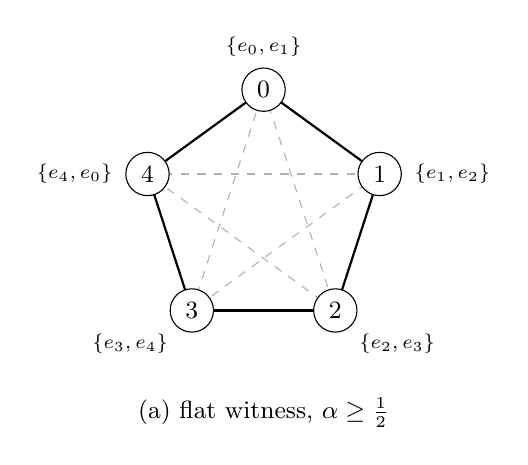
\begin{tikzpicture}[v/.style={circle, draw, fill=white, inner sep=1.5pt,
                              minimum size=0.55cm, font=\small}]
\foreach \i in {0,...,4} {
  \coordinate (p\i) at ({90-72*\i}:1.55);
}
\foreach \i/\j in {0/2,1/3,2/4,3/0,4/1}
  \draw[gray!60, dashed] (p\i) -- (p\j);
\foreach \i/\j in {0/1,1/2,2/3,3/4,4/0}
  \draw[thick] (p\i) -- (p\j);
\foreach \i in {0,...,4} {
  \node[v] at (p\i) {$\i$};
}
\node[font=\scriptsize, anchor=south] at ($(p0)+(0,0.3)$) {$\{e_0,e_1\}$};
\node[font=\scriptsize, anchor=west]  at ($(p1)+(0.32,0)$) {$\{e_1,e_2\}$};
\node[font=\scriptsize, anchor=north west] at ($(p2)+(0.18,-0.18)$) {$\{e_2,e_3\}$};
\node[font=\scriptsize, anchor=north east] at ($(p3)+(-0.18,-0.18)$) {$\{e_3,e_4\}$};
\node[font=\scriptsize, anchor=east]  at ($(p4)+(-0.32,0)$) {$\{e_4,e_0\}$};
\node[font=\small] at (0,-2.55) {(a) flat witness, $\alpha\ge\frac12$};
\end{tikzpicture}
\end{minipage}\hfill
\begin{minipage}[b]{0.5\textwidth}
\centering
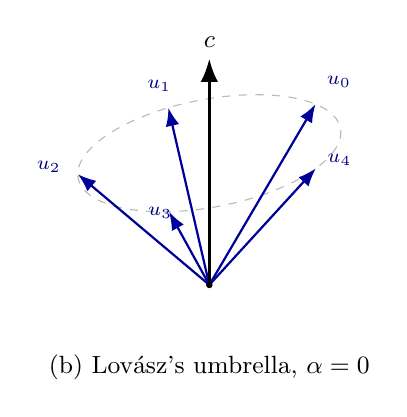
\begin{tikzpicture}[x={(2.1cm,0cm)}, y={(0.8cm,1.0cm)}, z={(0cm,2.5cm)},
                    >=Latex]
\pgfmathsetmacro{\cg}{5^(-0.25)}
\pgfmathsetmacro{\sg}{sqrt(1-\cg*\cg)}
\draw[gray!55, dashed] plot[domain=0:360, samples=90, smooth]
   ({\sg*cos(\x)},{\sg*sin(\x)},{\cg});
\foreach \i in {0,...,4} {
  \pgfmathsetmacro{\a}{72*\i+57}
  \draw[->, thick, blue!60!black] (0,0,0) -- ({\sg*cos(\a)},{\sg*sin(\a)},{\cg});
  \node[font=\scriptsize, blue!50!black] at ({1.22*\sg*cos(\a)},{1.22*\sg*sin(\a)},{\cg+0.06}) {$u_{\i}$};
}
\draw[->, very thick] (0,0,0) -- (0,0,1.15) node[above, font=\small] {$c$};
\fill (0,0,0) circle (1.2pt);
\node[font=\small] at (0,0,-0.42) {(b) Lov\'asz's umbrella, $\alpha=0$};
\end{tikzpicture}
\end{minipage}
\caption{Two optimal geometries for the pentagon.  Solid lines are edges and
dashed chords are the non-edges, which must be orthogonal.  (a) Vertex $i$ gets
the uniform state on $\{e_i,e_{i+1}\}$ and the center is $I/5$.  Non-adjacent
supports are disjoint, and the radius is $\log\frac52$ at every order.  (b)
Unit vectors $u_i$ on a cone around the handle $c$ with
$|\langle c,u_i\rangle|^2=1/\sqrt5$ and $u_i\perp u_{i+2}$.  This attains
$\vt(C_5)=\sqrt5$ at order zero, and its radius grows like
$5^{1/(2-2\alpha)}$.  Neither geometry is optimal for $0<\alpha<\frac12$.}
\label{fig:pentagon-geometries}
\end{figure}

\subsection{Below order one half}

Order zero is governed by a trace-norm version of \cref{lem:hs}, with the
constant $\sqrt5$ in place of $2$.  Interpolating between the two gives
everything in between.

\begin{lemma}[trace-norm inequality]\label{lem:trace}
For every representation of $C_5$ and every operator $X$,
$\sum_i\nrm{P_iXP_i}_1\le\sqrt5\,\nrm X_1$.
\end{lemma}

\begin{proof}
If $(P_i)$ represents $G$ and $v$ is a vector, pick unit vectors
$u_i\in\ran P_i$ parallel to $P_iv$ (arbitrary if $P_iv=0$).  They form an
orthonormal representation of $G$, and $\sum_i\nrm{P_iv}^2=\sum_i|\langle
u_i,v\rangle|^2\le\vt(\overline G)\nrm v^2$ by Lov\'asz's theorem
\cite{Lovasz1979}.  The pentagon is self-complementary, so the constant is
$\sqrt5$.  For $X=ab^*$ we have $\nrm{P_iab^*P_i}_1=\nrm{P_ia}\nrm{P_ib}$, and
Cauchy--Schwarz proves the claim for rank one.  A singular value decomposition
and the triangle inequality do the rest.
\end{proof}

\begin{lemma}[interpolation]\label{lem:interp}
For $1\le p\le2$, every representation of $C_5$ and every operator $X$,
\[
 \sum_i\nrm{P_iXP_i}_p^p\le B(p)\,\nrm X_p^p,
 \qquad B(p)=5^{(2-p)/2}\,2^{p-1}.
\]
\end{lemma}

\begin{proof}
The map $X\mapsto(P_iXP_i)_i$ has norm at most $\sqrt5$ from $S_1$ to
$\ell_1(S_1)$ by \cref{lem:trace}, and at most $\sqrt2$ from $S_2$ to
$\ell_2(S_2)$ by \cref{lem:hs}.  Complex interpolation of Schatten classes and
their $\ell_p$-sums \cite{BerghLofstrom1976,Bhatia1997} bounds its norm from
$S_p$ to $\ell_p(S_p)$ by $5^{(2-p)/(2p)}2^{(p-1)/p}$.  Raise this to the
power $p$.
\end{proof}

\begin{theorem}\label{thm:pentagon-bounds}
For $0\le\alpha\le\frac12$ and $p=1/(1-\alpha)$, the bounds
\eqref{eq:pentagon-intro} hold.
\end{theorem}

\begin{proof}
For the lower bound put $s=1/p$ and $X=\sigma^s$ in \cref{lem:interp}.  Then
$\nrm X_p^p=\Tr\sigma=1$ and $\nrm{P_i\sigma^sP_i}_p^p=Z_s(\sigma,P_i)$, so
$\sum_iZ_s(\sigma,P_i)\le B(p)$.  The minimum is at most the average, so
$\vt_\alpha(C_5)\ge5/B(p)=\sqrt5(\sqrt5/2)^{p-1}$.

The bound $\frac52$ is \cref{thm:pentagon-half} combined with monotonicity.
For the other upper bound, take the umbrella of
\cref{fig:pentagon-geometries}(b): unit vectors
$u_i=(\cos\gamma,\sin\gamma\cos\frac{2\pi i}5,\sin\gamma\sin\frac{2\pi i}5)$
with $\cos^2\gamma=1/\sqrt5$, which satisfy $u_i\perp u_{i+2}$.  For a pure
state, $\Tr\proj{u}^\alpha\sigma^{1-\alpha}=\bra u\sigma^{1-\alpha}\ket u$.
As faithful centers approach $\proj c$ with $c=(1,0,0)$, this tends to
$|\langle c,u_i\rangle|^2=5^{-1/2}$ because $1-\alpha>0$.  The radius
therefore tends to $\frac{1}{1-\alpha}\log\sqrt5=\log5^{p/2}$.
\end{proof}

\subsection{A continuum of spectral points}

\begin{proof}[Proof of \cref{thm:B}]
The values on $[\frac12,2]$ are \cref{thm:pentagon-half}, and the bounds on
$[0,\frac12]$ are \cref{thm:pentagon-bounds}.  By
\cref{prop:continuity,prop:endpoints}, $\alpha\mapsto\vt_\alpha(C_5)$ is
continuous and nondecreasing on $[0,\frac12]$.  It runs from $\vt(C_5)=\sqrt5$
to $\frac52$, so by the intermediate value theorem its image is
$[\sqrt5,\frac52]$.  Parameters with different values on $C_5$ are different
functions, and each of them lies in $\Xs$ by \cref{thm:A}.
\end{proof}

The lower bound in~\eqref{eq:pentagon-intro} exceeds $\sqrt5$ as soon as
$\alpha>0$.  So no $\vt_\alpha$ with $\alpha>0$ equals $\vt$.

\begin{remark}[an explicit ladder]
Readers who want explicit separations without the intermediate value theorem
can use $\alpha_k=1/(8^{k+1}+1)$, $k\ge0$.  Then $p_k-1=8^{-(k+1)}$, and the
bounds~\eqref{eq:pentagon-intro} give
$\vt_{\alpha_{k+1}}(C_5)\le\sqrt5\cdot5^{(p_k-1)/16}
<\sqrt5\,(\sqrt5/2)^{p_k-1}\le\vt_{\alpha_k}(C_5)$.  The strict inequality is
$5^{1/16}<\sqrt5/2$, that is, $2^{16}=65536<78125=5^7$.  Together with
$\vt_{\alpha_0}(C_5)\le5^{9/16}<\frac52$, this shows that
$\vt,\vt_{\alpha_0},\vt_{\alpha_1},\dots,\vt_{1/2}$ are pairwise distinct.
\end{remark}

\subsection{The Duan--Winter chain}\label{sec:dw-chain}

Duan and Winter prove the chain~\eqref{eq:dw-chain}
\cite[Eq.~(54)]{DuanWinter2016}.  They show that its last link can be strict,
and they conjecture that on the pentagon every term except the first equals
$\log\frac52$.  They also ask whether the two middle links can ever be strict.
We can now answer all of this.

\begin{corollary}[the pentagon conjecture]\label{cor:pentagon}
$\log\sqrt5<\Cmin(C_5)=\SNS(C_5)=\log\Sigma(C_5)=\log\alpha^*(C_5)=\log\frac52$.
\end{corollary}

\begin{proof}
\Cref{thm:pentagon-half,prop:endpoints} give
$\Cmin(C_5)=\log\Sigma(C_5)=\log\frac52$, and~\eqref{eq:dw-chain} squeezes
$\SNS(C_5)$ between them.  The fractional packing number of $C_5$ is
$\frac52$ and $\vt(C_5)=\sqrt5$ \cite{Lovasz1979}.
\end{proof}

This proof uses only \cref{lem:hs}, the projection formula and
monotonicity in $\alpha$.  The product theorem is not needed for the pentagon,
but it is needed for the general statement.

\begin{corollary}[the middle links]\label{cor:middle}
For every graph $G$, $\SNS(G)=\log\Sigma(G)$.  There is a graph with
$\Cmin(G)<\SNS(G)$.
\end{corollary}

\begin{proof}
The first statement is \cref{rem:single-letter}.  The second is
\cref{thm:C}, since $\Cmin(G_{32})<\log\Sigma(G_{32})=\SNS(G_{32})$.
\end{proof}

Duan and Winter also ask whether $\Sigma$ can be strictly submultiplicative
\cite{DuanWinter2016}.  For confusability graphs, with the optimization over
compatible channels built in, \cref{thm:product} says that it cannot.  Their
question for general non-commutative bipartite graphs is not addressed here.

\section{Order one versus order two}\label{sec:small}

\subsection{Where to look}

\Cref{lem:flat} tells us where \emph{not} to look.  If some flat witness is
optimal at order one, then orders one and two agree.  This is what happens on
the pentagon, and on every graph whose best order-one channel is flat.  To
separate the endpoints we need a graph whose good channels are genuinely
quantum.  Contextuality scenarios are a natural source, since they come with
rigid noncommutative representations.  We take the most familiar one, the
Mermin--Peres magic square \cite{Mermin1990,Peres1990}, and then add weights
by cloning vertices.  This section works directly from the definitions
\eqref{eq:cmin-def} and~\eqref{eq:sigma-def} and does not use
\cref{thm:product}.

\subsection{The graph}

\begin{figure}[t]
\centering
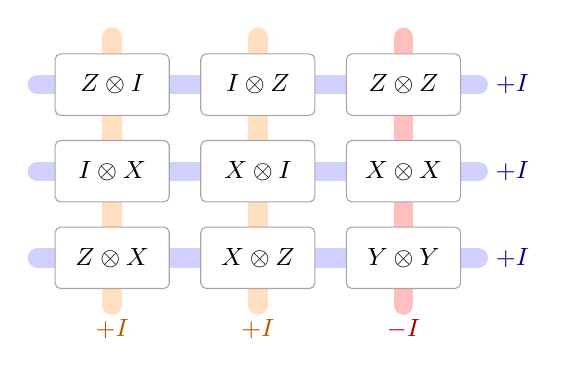
\begin{tikzpicture}[cell/.style={draw=gray!70, fill=white, rounded corners=2pt,
     minimum width=1.45cm, minimum height=0.78cm, font=\small}]
\def\cx{1.85}\def\cy{1.1}
\foreach \r in {0,1,2}
  \draw[line width=7pt, blue!18, line cap=round] (-0.95,-\cy*\r) -- (2*\cx+0.95,-\cy*\r);
\foreach \c in {0,1}
  \draw[line width=7pt, orange!25, line cap=round] (\cx*\c,0.6) -- (\cx*\c,-2*\cy-0.6);
\draw[line width=7pt, red!25, line cap=round] (2*\cx,0.6) -- (2*\cx,-2*\cy-0.6);
\node[cell] at (0,0)            {$Z\otimes I$};
\node[cell] at (\cx,0)          {$I\otimes Z$};
\node[cell] at (2*\cx,0)        {$Z\otimes Z$};
\node[cell] at (0,-\cy)         {$I\otimes X$};
\node[cell] at (\cx,-\cy)       {$X\otimes I$};
\node[cell] at (2*\cx,-\cy)     {$X\otimes X$};
\node[cell] at (0,-2*\cy)       {$Z\otimes X$};
\node[cell] at (\cx,-2*\cy)     {$X\otimes Z$};
\node[cell] at (2*\cx,-2*\cy)   {$Y\otimes Y$};
\foreach \r in {0,1,2}
  \node[font=\small, blue!55!black, anchor=west] at (2*\cx+1.05,-\cy*\r) {$+I$};
\node[font=\small, orange!70!black] at (0,-2*\cy-0.9)   {$+I$};
\node[font=\small, orange!70!black] at (\cx,-2*\cy-0.9) {$+I$};
\node[font=\small, red!65!black]    at (2*\cx,-2*\cy-0.9) {$-I$};
\end{tikzpicture}
\caption{The Mermin--Peres magic square.  Each row and each column is a
\emph{context}: its three observables commute, and their product is the
operator shown at its end.  A vertex of the seed graph $F$ is a context
together with a joint eigenvalue pattern (three signs with the prescribed
product).  That gives four vertices per context and $24$ in all.}
\label{fig:magic}
\end{figure}

Index the nine cells of a $3\times3$ array by $(i,j)\in\{0,1,2\}^2$, and fill
them with the two-qubit observables of \cref{fig:magic}.  The six contexts are
the three rows and the three columns.  A vertex of the \emph{seed graph} $F$
is a context together with signs for its three cells: signs with product $+1$
on rows and on the first two columns, and with product $-1$ on the last
column.  Two distinct vertices are non-adjacent if they belong to the same
context, or if they give opposite signs to a shared cell.  That makes
$24$ vertices, each non-adjacent to exactly nine others ($216$ ordered
non-adjacent pairs).

For a context whose first two observables are $A$ and $B$, the vertex with
first two signs $(s,t)$ is represented by the joint eigenprojection
\[
 Q_{A,B;s,t}=\tfrac14(I+sA)(I+tB),
\]
a rank-one projection on $\mathbb C^2\otimes\mathbb C^2$.  These projections
represent $F$.  In fact $Q_vQ_w=0$ holds exactly for the non-adjacent pairs,
with no accidental orthogonality.  Let vertex $0$ be the first-row vertex
with signs $(+,+,+)$, so $Q_0=\proj{00}$, and sort the vertices by overlap
$j_v=4\Tr Q_vQ_0\in\{0,1,2,4\}$.  The four classes have sizes $9,8,6,1$.
Class $0$ consists of the nine non-neighbours of vertex $0$, and class $4$ is
vertex $0$ itself.

Weights enter through cloning.  For a profile $k=(k_0,k_1,k_2,k_4)$ of
nonnegative integers, the \emph{clone graph} $F[k]$ replaces every class-$j$
vertex by $k_j$ pairwise non-adjacent copies (deleting it if $k_j=0$).  Each
copy inherits its parent's adjacencies to all other vertices.  Our main
example is
\[
 G_{32}=F[(2,1,1,0)],\qquad |V(G_{32})|=2\cdot9+8+6=32 .
\]

\subsection{Two weights and a bridge}

Two of the weights of \cref{sec:compressions} matter here.  The Gibbs weight
$w_\sigma(P)=Z_0(\sigma,P)$ belongs to order one, and the harmonic weight
$h_\sigma(P)=Z_{-1}(\sigma,P)=\Tr\sigma_{/P}$ belongs to order two.  For a
profile $k$, let $t_W(F[k])$ be the supremum of
$\min_{v:\,k_v>0}w_\sigma(P_v)/k_v$ over representations $(P_v)$ of the seed
$F$ and faithful states $\sigma$.  Define $t_H(F[k])$ in the same way with
$h_\sigma$.  Here $k_v$ means $k_{j_v}$, and deleted vertices may be
represented by $P_v=0$.

\begin{proposition}[bridge]\label{prop:bridge}
For every profile $k$,
\[
 2^{\Cmin(F[k])}\le\frac1{t_W(F[k])}
 \qquad\text{and}\qquad
 \Sigma(F[k])\ge\frac1{t_H(F[k])} .
\]
\end{proposition}

\begin{proof}
\emph{Upper bound on $\Cmin$.}  Start from a representation $(P_v)$ of $F$
and a state $\sigma$.  Let $A=\prod_{v:k_v>0}\{1,\dots,k_v\}$, work on
$\bigoplus_{f\in A}\cH$, and put
\[
 \sigma'=\frac1{|A|}\bigoplus_{f\in A}\sigma,\qquad
 P'_{v,a}=\bigoplus_{f\in A:\,f(v)=a}P_v
\]
(zero in the other summands).  Copies of one vertex live in disjoint sets of
summands, so they are orthogonal, and non-adjacent seed vertices stay
orthogonal.  So $(P'_{v,a})$ represents $F[k]$.  Functional calculus on the
direct sum gives $w_{\sigma'}(P'_{v,a})=w_\sigma(P_v)/k_v$.  Now apply the
projection formula~\eqref{eq:projection-formula} at $\alpha=1$ together with
$\vt_1=2^{\Cmin}$.

\emph{Lower bound on $\Sigma$.}  Take a compatible family $(\rho_{v,a})$ for
$F[k]$ and $T\ge\rho_{v,a}$, put $t=\Tr T$ and $\sigma=T/t$ (regularized if
needed), and let $P_{v,a}$ be the supports.  As in
\cref{prop:endpoints}, $h_\sigma(P_{v,a})\ge1/t$.  Copies of one vertex are
non-adjacent, so $P_v=\sum_aP_{v,a}$ is a projection, and $(P_v)$ (with
$P_v=0$ for deleted $v$) represents $F$.  The harmonic weight is
superadditive over orthogonal blocks: for a positive definite block matrix
$M$, each diagonal block of $M^{-1}$ dominates the inverse of the
corresponding block of $M$.  Applied to $M=P_v\sigma^{-1}P_v$ this gives
$h_\sigma(P_v)\ge\sum_ah_\sigma(P_{v,a})\ge k_v/t$.  Hence
$t_H(F[k])\ge1/t$.
\end{proof}

The upper bound on $\Cmin$ needs one good witness.  The lower bound on
$\Sigma$ needs an upper bound on $t_H$ valid for \emph{every} representation,
in every dimension.  That is the job of the next subsection.

\subsection{Harmonic weights as moments}

Let $(P_v)$ represent $F$ on $\cH$ and let $\sigma$ be faithful.  Put
$\Omega=\vect(\sqrt\sigma)\in\cH\otimes\cH$, let $F_v$ be the orthogonal
projection onto $\sigma^{-1/2}\ran P_v$, and let $E_v=F_v^{\mathsf T}$.

\begin{lemma}[harmonic weight as a moment]\label{lem:harmonic-moment}
For every $v$,
\[
 (P_v\otimes E_v)\Omega=(I\otimes E_v)\Omega
 \qquad\text{and}\qquad
 \langle\Omega,(I\otimes E_v)\Omega\rangle=h_\sigma(P_v).
\]
\end{lemma}

\begin{proof}
With $(A\otimes B)\vect(M)=\vect(AMB^{\mathsf T})$, the first identity says
$P_v\sqrt\sigma F_v=\sqrt\sigma F_v$.  This holds because $\sqrt\sigma F_v$
has range $\ran P_v$.  For the second, $\sqrt\sigma F_v\sqrt\sigma$ lies below
$\sigma$ and has range in $\ran P_v$.  If $0\le A\le\sigma$ has range in
$\ran P_v$, then $\sigma^{-1/2}A\sigma^{-1/2}$ is a contraction supported in
$\ran F_v$, hence at most $F_v$.  So
$\sqrt\sigma F_v\sqrt\sigma=\sigma_{/P_v}$, and its trace is the moment.
\end{proof}

So harmonic weights are expectations in the vector $\Omega$ of two commuting
families of projections, $P_v\otimes I$ and $I\otimes E_w$.  The first family
obeys the orthogonality relations of $F$.  The second obeys no relations of its
own, but it is tied to the first by the identity of
\cref{lem:harmonic-moment}.  This is exactly the setting of noncommutative
moment relaxations \cite{NPA2008,Mghirbi2026}.  We form the Gram matrix of the
$409$ vectors
\[
 \Omega,\quad (P_a\otimes I)\Omega,\quad (I\otimes E_b)\Omega,\quad
 (P_a\otimes E_b)\Omega\ \ (a=b\text{ or }a\sim b).
\]
The pairs with $a\not\simeq b$ are left out because those vectors vanish:
$(P_a\otimes E_b)\Omega=(P_aP_b\otimes E_b)\Omega=0$.  The Gram matrix is
positive semidefinite, its corner entry is $\Tr\sigma=1$, and the entry
$\langle\Omega,(I\otimes E_v)\Omega\rangle$ is $h_\sigma(P_v)$.  Many entries
coincide or vanish in every model.  We record these coincidences in a table
of $1009$ moment keys, using four rewriting rules together with symmetry
(\cref{app:certificate}).  Maximizing $t$ subject to positivity, the corner
normalization and $h_v\ge tk_v$ gives an upper bound on $t_H(F[k])$ in every
dimension.  A rational dual solution then certifies a rational upper bound.

\subsection{Certified values}

\begin{table}[t]
\centering
\begin{tabular}{@{}lcrccc@{}}
\toprule
graph & profile $(k_0,k_1,k_2,k_4)$ & vertices & $2^{\Cmin}\le$ & $\Sigma\ge$ & gap (bits)\\
\midrule
$G_{32}$ & $(2,1,1,0)$ & 32 & $6.186983\ldots$ & $6.194232\ldots$ & $0.001689$\\
$G_{44}$ & $(1,2,3,1)$ & 44 & $8.949075\ldots$ & $8.962394\ldots$ & $0.002146$\\
$G_{72}$ & $(4,3,2,0)$ & 72 & $105/8$          & $13.191800\ldots$ & $0.007324$\\
\bottomrule
\end{tabular}
\caption{Certified bounds for three clone graphs.  Upper bounds on
$2^{\Cmin}$ come from explicit rational Gibbs witnesses: a direct sum of the
magic-square representation and one-dimensional clique representations.
Lower bounds on $\Sigma$ come from rational dual certificates for the moment
relaxation.}
\label{tab:certified}
\end{table}

\Cref{tab:certified} lists the certified bounds.  For $G_{32}$ the exact
rational values are
\begin{equation}\label{eq:g32-rationals}
 t_W(G_{32})\ \ge\ \frac{5225365592240894}{32329248967670751}
 \ >\ \frac{15147154828811}{93824992214030}\ \ge\ t_H(G_{32}).
\end{equation}
For $G_{44}$ and $G_{72}$ the certified harmonic bounds are
$t_H\le31406288103814/281475531618259$ and
$t_H\le21337116511217/281474976708840$.

\begin{proof}[Proof of \cref{thm:C}]
Combine~\eqref{eq:g32-rationals} with \cref{prop:bridge}.  The reciprocals of
the two rationals are $6.186983\ldots$ and $6.194232\ldots$.
\end{proof}

\section{Open problems}\label{sec:open}

\paragraph{Is $\vt$ the least point?}
Every $\vt_\alpha$ dominates $\vt$, so this paper leaves the conjecture
$\Theta_*=\vt$ where it was.  A proof that $\vt$ is the minimum of $\Xs$ would
settle it.  So would a single spectral point below $\vt$ on some graph, in the
opposite direction.

\paragraph{Above order two.}
\Cref{rem:above-two} shows that our monotonicity argument breaks down above
order two.  Is some suitably defined $\vt_\alpha$ with $\alpha>2$ still in
$\Xs$?  Flat witnesses show that any such extension is at most $\alpha^*$.
A natural guess for the $\alpha\to\infty$ endpoint is the complement of the
projective rank.  Flat representations give the corresponding upper bound, but
we are missing a dimension-free argument for the other direction.

\paragraph{Other divergences.}
The proof of \cref{thm:A} uses three features of the Petz family.  These are
a closed form for the supported minimum with the tower property, the
block structure used for unions and flagged mixtures, and data processing.
For sandwiched divergences of order $\beta\ge1$ the question has a complete
answer: by \cref{prop:sandwiched} they reproduce the Petz curve on $[1,2]$,
from $2^{\Cmin}$ at $\beta=1$ to $\Sigma$ at $\beta=\infty$.  Sandwiched
divergences also satisfy data processing for $\frac12\le\beta<1$
\cite{Tomamichel2016}, but there we have no closed form for the supported
minimum.  Do these orders give spectral points, and do they differ from the
$\vt_\alpha$ with $\alpha<1$?

\paragraph{Convexity.}
In the ordinary spectrum, Vrana's probabilistic refinement makes the spectrum
log-convex \cite{Vrana2021}.  If the same held for $\le_*$, interpolating
between $\vt$ and $\Sigma$ would produce another continuum.  At least part of
the R\'enyi family is not of this form.  Along such interpolations,
vertex-transitive graphs are evaluated log-affinely \cite{Vrana2022}.  A point
with value $\frac52$ on $C_5$ would then carry no weight on $\vt$, so it would
be $\Sigma$ itself.  But $\vt_1(C_5)=\frac52$ and $\vt_1\ne\Sigma$ by
\cref{thm:C}.  So $\vt_1$ is not such an interpolant, and we do not know
whether the $\vt_\alpha$ with $\alpha<\frac12$ are.  Making any of this
rigorous would need an entanglement-assisted theory of probabilistic
refinements, which we do not have.

\paragraph{The pentagon curve.}
What is $\vt_\alpha(C_5)$ for $0<\alpha<\frac12$?  The bounds in
\cref{fig:pentagon-curve} do not meet, and neither geometry in
\cref{fig:pentagon-geometries} is optimal there.

\paragraph{Small separations.}
How small can a graph with $\Cmin<\log\Sigma$ be?  Thirty-two vertices
suffice, and we have no reason to think this is minimal.  Can the rational
certificate behind \cref{thm:C} be replaced by a short analytic inequality,
in the spirit of \cref{lem:hs}?  And is the first level of the moment
relaxation already exact for the three graphs of \cref{tab:certified}?

\paragraph{Non-commutative graphs.}
Duan, Severini and Winter's quantum Lov\'asz number extends $\vt$ to
non-commutative graphs \cite{DSW2013}.  Does the whole family $\vt_\alpha$
extend, and does the product theorem survive?  A positive answer at order two
would bear on Duan and Winter's question about strict submultiplicativity of
$\Sigma$ for general non-commutative bipartite graphs.

\paragraph{Reproducibility.}
The certificate data and the verification scripts accompany this paper.
They are needed only for the finite rational claims of \cref{sec:small}.
Everything else is proved in the text.

\paragraph{AI-assisted tools.}
Generative AI tools were used throughout the research and preparation of this
manuscript, including for mathematical exploration, proof development and
critique, literature organization, computational assistance, and drafting.
The authors determined which results and arguments to include and take
responsibility for the final manuscript.  Exact computer-assisted claims are
supported, where indicated, by accompanying deterministic certificates and
verification scripts.

\appendix

\section{The certificate}\label{app:certificate}

\paragraph{Words and moments.}
For words $L=a_1\cdots a_m$ and $R=b_1\cdots b_n$ in seed vertices, write
$P_L=P_{a_1}\cdots P_{a_m}$, $E_R=E_{b_1}\cdots E_{b_n}$ and
\[
 m(L,R)=\langle\Omega,(P_L\otimes E_R)\Omega\rangle .
\]
Every entry of the Gram matrix of \cref{sec:small} is such a moment.  The
following rules hold in every model.
\begin{enumerate}[label=(R\arabic*),leftmargin=2.6em,itemsep=1pt]
\item Equal adjacent letters in $L$ or in $R$ merge, since $P_a^2=P_a$ and
$E_b^2=E_b$.
\item If $L$ contains two adjacent letters $a\ne b$ that are non-adjacent in
$F$, then $m(L,R)=0$, since $P_aP_b=0$.
\item If $R$ ends in $y$, then $m(L,R)=m(Ly,R)$, since
$(I\otimes E_y)\Omega=(P_y\otimes E_y)\Omega$.
\item If $R$ begins with $y$, then $m(L,R)=m(yL,R)$, by the adjoint of the
same identity.
\end{enumerate}
Reversing both words conjugates the moment, since
$(P_L\otimes E_R)^*=P_{\bar L}\otimes E_{\bar R}$.  Let $\mathcal A_0$ be the
$48$ automorphisms of $F$ that fix vertex $0$ (equivalently, that preserve
the overlap classes).  A relabelled representation is again a representation,
and the constraints $h_v\ge tk_v$ are invariant because $k$ is constant on
classes.  So we may average the Gram matrix over $\mathcal A_0$ and then take
real parts.  Both operations preserve positivity, and together they identify
symmetry-related moments and reversed pairs.  The verifier builds the key
table from these rules only.  So every identification in the table holds for
the Gram matrix of every representation, in every dimension.  The result has
$1009$ keys.

\paragraph{Deleted vertices.}
In $G_{32}$ and $G_{72}$ the class-$4$ vertex is deleted.  It stays in the
seed and is represented by $P_0=0$, and hence $E_0=0$.  All four rules remain
valid for zero projections, no radial constraint is imposed on deleted
vertices, and the relaxation needs no change.

\paragraph{The relaxation and its dual.}
Let $\Gamma(y)$ be the real symmetric matrix with one variable $y_\kappa$ per
key, and let $\kappa_v$ be the key of $m(\varnothing,v)=h_\sigma(P_v)$.  The
primal problem is to maximize $t$ subject to
\[
 \Gamma(y)\succeq0,\qquad y_1=1,\qquad y_{\kappa_v}\ge tk_v\ \ (k_v>0).
\]
A dual certificate consists of $Z\succeq0$, multipliers $\mu_v\ge0$ and a
number $\lambda$ such that, for every key $\kappa$,
\begin{equation}\label{eq:moment-dual}
 \sum_{(i,j):\,\mathrm{key}(i,j)=\kappa}Z_{ij}
 +\sum_{v:\,\kappa_v=\kappa}\mu_v=\lambda\,[\kappa=1].
\end{equation}
Pairing with $\Gamma(y)$ gives
$0\le\langle Z,\Gamma(y)\rangle=\lambda-\sum_v\mu_vy_{\kappa_v}$, and
therefore
\[
 t_H(F[k])\le\frac{\lambda}{\sum_v\mu_vk_v}.
\]

\paragraph{Exact positivity.}
The file \texttt{certificates/small\_graph\_certificates.json} contains, for
each graph, the rational Gibbs witness, the multipliers $\mu$, and the nonzero
orbits of $Z$.  The verifier rebuilds the seed, its $216$ ordered non-adjacent
pairs, the two-qubit representation, the overlap classes, the $48$
automorphisms, the $409$ monomials and the key table.  It checks
every equation~\eqref{eq:moment-dual} and $\mu\ge0$ in rational arithmetic,
and it recomputes the Gibbs witness exactly.  To prove $Z\succeq0$, it clears
denominators, $DZ\in\mathbb Z^{409\times409}$, rounds a floating-point
Cholesky factor at scale $2^{40}$ to an integer matrix $L$, and checks in
exact integer arithmetic that
\[
 R=2^{80}DZ-DLL^{\mathsf T}
\]
is symmetric and diagonally dominant with nonnegative diagonal.  Then
$R\succeq0$ and $Z=LL^{\mathsf T}/2^{80}+R/(2^{80}D)\succeq0$.  Only the
integer check counts.  Whether the floating-point factorization succeeded
plays no role.

\paragraph{Negative controls.}
The verifier runs two tampered certificates, and both must be rejected.  One
breaks an affine equation.  The other changes only entries attached to moments
that vanish identically, so every affine equation still holds but exact
positivity fails.

\paragraph{How the certificate was found.}
We followed the recovery procedure of \cite{Mghirbi2026}.  A numerical SDP
solution is symmetrized, rounded to dyadic rationals, and projected exactly
onto the affine constraints by a minimum-norm correction, and positivity is
then certified as above.  None of this matters for correctness, which rests
only on the exact checks.

\section{Deferred proofs}\label{app:proofs}

\subsection{Continuity in the order}\label{app:continuity}

\begin{proof}[Proof of \cref{prop:continuity}]
Write $f(\alpha)=\log\vt_\alpha(G)$.

\emph{Right continuity at $\alpha_0\in[0,1)$.}  Pick a compatible family and
a faithful center whose order-$\alpha_0$ radius is at most $f(\alpha_0)+\eps$.
For fixed states with a faithful center, $\alpha\mapsto D_\alpha$ is
continuous on $[0,1)$, including from the right at $0$, because
$\rho^\alpha\to\Pi_\rho$.  So
$\limsup_{\alpha\downarrow\alpha_0}f(\alpha)\le f(\alpha_0)+\eps$, and
monotonicity gives the reverse inequality.

\emph{Left continuity at $\alpha\in(0,1)$.}  Let $0<\beta<\alpha$ and
$\psi(t)=\ln\Tr\rho^t\sigma^{1-t}$.  By H\"older's inequality $\psi$ is
convex, and $\psi(1)=0\ge\psi(0)$.  So
$\psi(\beta)\le(1-\frac\beta\alpha)\psi(0)+\frac\beta\alpha\psi(\alpha)
\le\frac\beta\alpha\psi(\alpha)$.  Since both orders lie below one, this
rearranges to
\[
 D_\alpha(\rho\Vert\sigma)\le\frac{\alpha(1-\beta)}{\beta(1-\alpha)}
 D_\beta(\rho\Vert\sigma).
\]
The constant does not depend on the states or the dimension.  Applying it to
near-optimal witnesses at order $\beta$ gives
$f(\beta)\le f(\alpha)\le\frac{\alpha(1-\beta)}{\beta(1-\alpha)}f(\beta)$,
and the constant tends to $1$ as $\beta\uparrow\alpha$.
\end{proof}

\subsection{Orthogonal blocks}\label{app:orthogonal-sum}

\begin{proof}[Proof of \cref{lem:orthogonal-sum}]
For $s\ne0$ let $A=\sigma^s$ and $f(t)=t^{1/s}$.  For $s=0$ let $A=\ln\sigma$
and $f=\exp$.  In each case $f$ is convex on the spectrum of $A$ and
$f(A)=\sigma$.  Diagonalize $Q_jAQ_j$ on $\ran Q_j$ in an orthonormal basis
$(e_{jk})_k$.  Its eigenvalues are $\langle e_{jk},Ae_{jk}\rangle$, so
Jensen's inequality for the spectral measure of $A$ gives
\[
 Z_s(\sigma,Q_j)=\sum_kf(\langle e_{jk},Ae_{jk}\rangle)
 \le\sum_k\langle e_{jk},\sigma e_{jk}\rangle .
\]
The vectors $(e_{jk})_{j,k}$ are orthonormal, so the total is at most
$\Tr\sigma=1$.
\end{proof}

\subsection{Exact confusability graphs}\label{app:exact}

\begin{lemma}\label{lem:exact-graph}
In~\eqref{eq:def-parameter}, \eqref{eq:cmin-def} and~\eqref{eq:sigma-def},
restricting to channels whose confusability graph is exactly $G$ does not
change the infimum.
\end{lemma}

\begin{proof}
Restricting can only increase an infimum, so we show the reverse.  Take a
compatible family $(\rho_x)$ on $\cH$ with center $\sigma$ (or dominator
$T$).  If $E(G)=\varnothing$, every compatible family already has exact
confusability graph $G$, so there is nothing to prove.  Assume henceforth that
$|E(G)|>0$.  Add an orthonormal vector $f_e$ for each edge $e$ of $G$.  For a
vertex $x$ of degree $d_x>0$, let $\Pi_x$ project onto the $f_e$ with $e\ni x$,
and let $\Pi_E$ project onto all of them.  Put
\[
 \rho'_x=(1-\eps)\rho_x\oplus\frac{\eps}{d_x}\Pi_x,\qquad
 \sigma'=(1-\eps)\sigma\oplus\frac{\eps}{|E|}\Pi_E,\qquad
 T'=T\oplus\eps\,\Pi_E ,
\]
and leave isolated vertices unchanged.  Adjacent $x,y$ now overlap on
$f_{\{x,y\}}$, while non-adjacent vertices share no new vector.  So the
confusability graph is exactly $G$.  Every Petz moment, relative entropy and
support weight splits over the two summands, and the new summand contributes
$O(\eps)$.  So radii converge to the original ones as $\eps\to0$.  Also
$T'\ge\rho'_x$ and $\Tr T'\to\Tr T$.  The statement for $\Cmin$ follows from
the order-one radius identity.
\end{proof}

\bibliographystyle{alpha}
\bibliography{references}

\end{document}
